\documentclass{cjas_journal}

\TitleZH{耦合安全约束下多机器人协同脱困的包络等变图强化学习与邻域近端分配控制}
\AuthorsZH{谭\quad 为，\quad 陈\quad 鑫$^{\ast}$}
\AffilZH{中国地质大学（武汉）人工智能与自动化学院，湖北 武汉 430074；复杂系统先进控制与智能自动化湖北省重点实验室，湖北 武汉 430074}

\AbstractZH{针对全局标量连通保持与局部成对机间避碰两类相互冲突的耦合安全约束下，多机器人系统在密集对称交会中易陷入非目标几何死锁、外围静止邻居阻挡通道以及学习残差引发终点稳态悬停的问题，本文提出一种包络等变图策略与邻域近端分配（Envelope Equivariant Graph Policy with Neighborhood Proximal Allocation, EGP-NPA）协同控制方法。首先，构造七机器人对称接触构型的精确有理数二阶 Karush–Kuhn–Tucker（KKT）严格局部极小证书，从代数上证明即便全员可动且存在满足全程避碰与连通下界的显式安全可达路径，任何强制总位置误差单调不增（$\dot{W}\le 0$）的短视控制障碍函数（CBF）滤波器均被正定拉格朗日 Hessian 与球面二次能量壁垒锁死，并定量揭示“待互换节点侧向破对称标称驱动”与“外围静止邻居经由动态配额让渡协同退让”两项局部脱困物理机制。其次，构建满足平面特殊正交群 $\mathrm{SO}(2)$ 旋转、平移与节点置换等变的消息传递图神经网络（GNN）残差标称策略，证明手性旋转偏置对破除镜像共线死锁的结构必要性；接入基于反对称边记录与闭邻域块二次规划的邻域近端分配（NPA）安全护盾，导出接触边界上动态碰撞份额转移驱动外围静止邻居同向退让的显式严格正闭式解，并阐明在策略损失中惩罚法向滤波修正量削弱退让动力的代数机理；进一步提出仅依赖一跳目标距离的闭邻域完成包络，证明其在终点邻域将零阶成对排斥偏置一阶压制为 $\mathcal{O}(\lVert\boldsymbol{e}_k\rVert_2)$ 并精确恢复目标零速平衡点。最后，基于小规模短轮数（$N\in\{6,\dots,10\}, B=2$）多智能体近端策略优化（MAPPO）训练与大规模多轮（$N\in\{12,20,25\}, B=8$）零样本部署，EGP-NPA 在 $96$ 组密集三角晶格互换与全排列基准及 $48$ 组独立盲测实例上实现 $100\%$ 安全达标与零违约，跨规模安全达标率显著优于护盾投影一致性安全强化学习（$53.1\%$）、静态配额平摊 CBF 护盾图策略（$3.1\%$）、离散图障碍函数近端策略优化（DGPPO，$0\%$ 无违约达标）、原始—对偶拉格朗日安全强化学习（$0\%$ 无违约达标）、切向环流启发式（$40.6\%$）与短视比例吸引滤波（$15.6\%$），并通过同预算析因实验、固定权重单变量消融及 \texttt{MuJoCo} 二阶全向底盘虚拟物理闭环实验验证了方法的有效性与物理可通行性边界。}

\KeywordsZH{多机器人系统；耦合安全约束；控制障碍函数；安全强化学习；等变图神经网络；几何死锁；邻域近端分配}
\CLCCode{TP242; TP273}

\TitleEN{Envelope Equivariant Graph Reinforcement Learning and Neighborhood Proximal Allocation for Cooperative Deadlock Resolution of Multi-Robot Systems Under Coupled Safety Constraints}
\AuthorsEN{TAN Wei,\quad CHEN Xin$^{\ast}$}
\AffilEN{School of Artificial Intelligence and Automation, China University of Geosciences, Wuhan 430074, China; Hubei Key Laboratory of Advanced Control and Intelligent Automation for Complex Systems, Wuhan 430074, China}

\AbstractEN{To address non-target geometric deadlocks, channel blockage by outer stationary neighbors, and terminal steady-state hovering induced by learned residuals in multi-robot systems subject to mutually conflicting global connectivity and pairwise collision-avoidance scalar constraints, this paper proposes an Envelope Equivariant Graph Policy with Neighborhood Proximal Allocation (EGP-NPA) cooperative control framework. First, an exact rational second-order Karush--Kuhn--Tucker (KKT) certificate is constructed on a seven-robot symmetric contact configuration, proving algebraically that even when all robots are mobile and an explicit collision-free, connected path exists, any myopic Control Barrier Function (CBF) safety filter enforcing monotone error descent ($\dot{W}\le 0$) is trapped by a positive-definite Lagrangian Hessian over the critical cone and a finite-radius quadratic energy barrier. This certificate identifies two key physical mechanisms for deadlock resolution: lateral symmetry-breaking nominal drive from swapping robots and dynamic quota-driven yielding from outer stationary neighbors. Second, a planar $\mathrm{SO}(2)$ rotation-, translation-, and permutation-equivariant message-passing Graph Neural Network (GNN) residual nominal policy is constructed, proving the structural necessity of chiral rotational bias over $\mathrm{O}(2)$ reflection equivariance. Coupled with a closed-neighborhood block NPA safety shield with antisymmetric edge-ledger local settlement, we derive the explicit positive closed-form solution for pairwise quota transfer and stationary neighbor yielding velocity on contact boundaries, and show how penalizing normal filter intervention weakens cooperative yielding. Furthermore, a stateless one-hop closed-neighborhood completion envelope is proposed to suppress zero-order pairwise repulsive biases to $\mathcal{O}(\lVert\boldsymbol{e}_k\rVert_2)$ near the goal and restore the zero-velocity target equilibrium. Finally, trained via Multi-Agent Proximal Policy Optimization (MAPPO) on small teams ($N\in\{6,\dots,10\}, B=2$) and deployed zero-shot to larger teams ($N\in\{12,20,25\}, B=8$), EGP-NPA achieves $100\%$ safe arrival and zero safety violations across $96$ dense triangular-lattice swap/permutation benchmarks and $48$ independent holdout instances, outperforming shield-consistent safe MARL ($53.1\%$), static-split CBF shielded GNN ($3.1\%$), task-adapted Discrete GCBF Proximal Policy Optimization (DGPPO, $0\%$ violation-free arrival), primal-dual MAPPO-Lagrangian ($0\%$ violation-free arrival), tangential circulation heuristics ($40.6\%$), and myopic CBF filtering ($15.6\%$). Matched-budget factorial tests, fixed-weight ablations, and second-order \texttt{MuJoCo} simulations further validate each module and characterize the safety-margin versus channel-passability trade-off.}

\KeywordsEN{multi-robot systems; coupled safety constraints; control barrier functions; safe reinforcement learning; equivariant graph neural networks; geometric deadlock; neighborhood proximal allocation}

\FirstPageFootnote{收稿日期：2026-11-09.\quad 基金项目：国家自然科学基金资助项目.\quad 作者简介：谭为，博士研究生，主要研究方向为多机器人系统分布式估计、安全控制与强化学习；陈鑫（通信作者），教授，博士生导师，主要研究方向为复杂系统控制、多智能体协同与智能机器人，E-mail: chenxin@cug.edu.cn.}

\begin{document}
\makejournaltitle

\section{引言}\label{sec:intro}

在协同巡检、按需无线通信中继与密集编队重构等自主任务中，多机器人系统往往同时受制于两类方向相反、相互冲突的标量耦合安全约束：一方面，成对机间避碰约束要求相邻机器人之间保持安全排斥距离；另一方面，全局网络连通性保持约束（以图拉普拉斯代数连通度标量下界表征）将全网机器人耦合在一起，限制编队过度分散以防通信链路割裂\cite{yang2010decentralized,sabattini2013decentralized,ong2021connectivity}。控制障碍函数（Control Barrier Function, CBF）\cite{ames2017cbf,breeden2022sampled}通过将安全集前向不变性条件转化为关于控制输入的标量仿射不等式，为安全关键控制提供了高计算效率的二次规划（Quadratic Program, QP）滤波框架。针对包含全局耦合行与成对接触行的标量安全约束，现有研究已发展出基于连续时间无违约分布式梯度流\cite{tan2025violationfree}以及基于零和配额分解的邻域近端分配（Neighborhood Proximal Allocation, NPA）方法，使得多机器人系统在每个采样时刻仅凭有限轮一跳邻居通信即可获得严格满足全部耦合约束的安全控制输入。

然而，单拍安全滤波器的瞬时可行性并不蕴含长时程多机导航任务的完成性。当多台机器人在狭窄空间相向交会或需要在高密度阵列内部交换位置时，指向各自目标的标称吸引力往往被接触避碰约束与全局连通约束的法向反力同时抵消，使系统永久停滞在远离目标的对称平衡构型（即几何死锁，Geometric Deadlock）\cite{reis2021,grover2023deadlock,tan2024equilibria,mestres2026filters}。从物理与凸优化机制上看，传统 CBF 最小修正滤波器之所以在密集交会中频繁陷入死锁，根源在于其“逐拍单调降低原始位置误差”的短视结构。记全网机器人当前位置 $\bp$ 与固定标签目标 $\bg$ 的总欧氏位置误差为 $W(\bp)=\frac12\sum_{i=1}^N\norm{\bp_i-\bg_i}_2^2$。将指向目标的负梯度标称速度 $-k_g\nabla_{\bp}W=-k_g(\bp-\bg)$ 投影到包含零速度解的安全输入集上，必然强制要求 $\dot W(\bp(t))\le 0$\cite{allibhoy2024safegradient}。在内部节点迎面互换而外围邻居已处于各自目标位置（$\bp_j=\bg_j$）的密集编队中，这一单调性约束会产生双重锁死：其一，待互换节点的径向目标引力与直接接触避碰法向反力共线抵消，缺乏侧向破对称驱动；其二，外围静止邻居一旦暂时离开原位腾出几何通道就会导致总误差 $W(\bp)$ 短暂上升，且在静态配额平摊下其局部可行域在接触边界上直接坍缩为零\cite{karagoz2014navigation}。

为缓解安全滤波器引发的伪平衡点与死锁问题，现有文献主要探索了启发式切向环流与学习型安全控制两条技术路线。在解析控制方面，Reis 等\cite{reis2021}与 Tan 等\cite{tan2024equilibria}分析了单智能体及多智能体 CBF-QP 的非目标平衡点结构与鞍点不稳定性；Gon\c{c}alves 等\cite{goncalves2023circulation}与 Dai 等\cite{dai2024compatible}分别引入成对切向环流项与兼容控制李雅普诺夫—障碍函数（CLF-CBF）以打破单对接触下的共线停滞。然而，当内部互换节点被多层已达标的静止邻居紧密包裹时，无差别的常值环流会在多条接触边上引发旋转方向冲突，且在存在严格约束局部极小（而非鞍点）的对称接触构型下，任何依赖局部负曲率或要求 $W$ 单调不增的解析反馈均在数学上无法越过能量壁垒。在学习控制方面，原始—对偶拉格朗日约束多智能体强化学习（MAPPO-Lagrangian）\cite{gu2023safe}、预测与自适应安全滤波强化学习\cite{wabersich2021,liu2026saferl}、神经图控制障碍函数（GCBF+）\cite{zhang2025gcbf}及离散图策略近端优化（DGPPO）\cite{zhang2025dgppo}利用图神经网络（Graph Neural Network, GNN）学习多机协同与避碰策略。但现有多智能体安全强化学习方法仍面临三项悬而未决的结构性挑战：
\begin{enumerate}
 \item \textbf{全局与局部冲突耦合约束下的随时零违约保证缺失：} 神经障碍函数与软惩罚策略梯度仅能近似处理依赖局部相对坐标的成对避碰约束，无法在训练探索与有限通信轮数截断执行下严格保证全局标量连通约束 $\lambda_2(\bL(\bp))\ge\lr$ 与成对避碰约束在采样区间内的连续时间硬安全；
 \item \textbf{学习标称层与分布式动态配额分配层的脱节：} 现有安全护盾多采用单机独立投影或静态责任平摊（$B=0$），当外围机器人已到达自身目标（$\be_j=\boldsymbol 0$）时，静态平摊护盾会将其向外退让通道锁死，迫使学习策略在标称层同时拟合全部外围节点的退让轨迹，在多机密集接触下信用分配效率极低；
 \item \textbf{密集目标构型处的零阶排斥残差悬停：} 消息传递 GNN 输出的成对相对方向排斥项属于不随位置误差 $\be_k\to\boldsymbol 0$ 自动衰减的零阶偏置；在接触净空仅为毫米级的密集晶格终点处，持续非零的接触对偶乘子使冲突门控保持常开，导致机器人在目标微球外围发生持续稳态悬停与微幅抖振。
\end{enumerate}

针对上述挑战，本文提出包络等变图策略与邻域近端分配（Envelope Equivariant Graph Policy with Neighborhood Proximal Allocation, EGP-NPA）协同控制方法，将复杂的多机协同脱困问题解耦为“一跳等变图网络残差标称 + 闭邻域块动态分摊护盾 + 一跳闭邻域终点完成包络”三个紧密咬合的功能模块。本文的主要贡献归纳如下：
\begin{enumerate}
 \item \textbf{严格非目标局部极小的精确有理数二阶 KKT 证书与脱困物理机制（定理\ref{thm:seven-kkt}）：} 针对全员可动的七机器人双三角对称接触构型，利用有理数域代数闭合信道核与精确分数算术（$\mathbb Q$）构造原始—对偶 KKT 见证，严格证明拉格朗日 Hessian 在完整临界方向锥上一致正定（$\boldsymbol v^{\top}\boldsymbol H_L\boldsymbol v\ge\frac{19}{515}\norm{\boldsymbol v}_2^2$），并给出半径 $1/200$ 球面上的显式二次能量壁垒 $W(\bar\bp+\boldsymbol\delta)-W(\bar\bp)\ge\frac1{100}\norm{\boldsymbol\delta}_2^2>0$（在初态与目标均严格位于安全集内部的微扰开球上依然成立）及满足全程 $\lambda_2(\bL)\ge 1792/625>5/2$ 的解析可达路径。该证书从代数上排除了依靠鞍点负曲率或单调下降控制实现一般脱困的可能性，并定量揭示两项核心脱困物理机制：待互换节点的侧向破对称标称驱动与外围静止邻居经由动态配额让渡的协同退让。
 \item \textbf{手性旋转与置换等变的一跳图神经网络残差标称架构（命题\ref{prop:equivariance}）：} 在局部目标正交标架与有向边正交标架上构造融合几何投影与滤波器内部代数状态（单机重拟合碰撞影子价格 $\boldsymbol\mu_{i,k-1}$、谱配额与边记录）的两层参数共享消息传递 GNN，严格证明标称控制场对平面刚体变换群 $\mathrm{SO}(2)\ltimes\mathbb R^2$ 与节点置换群 $S_N$ 的等变性；同时从代数与实测两方面证明：保留特殊正交群 $\mathrm{SO}(2)$ 的确定性手性旋转偏置是打破镜像共线死锁的必要结构条件，若强制施加全正交群 $\mathrm{O}(2)$ 镜像反射等变，则在对称迎头交会构型上切向旋转输出必恒等于零（$\omega_{i,k}^\theta\equiv 0$）并退化回短视死锁。
 \item \textbf{闭邻域动态份额解冻闭式解与一跳闭邻域终点完成包络理论（命题\ref{prop:safety}--\ref{prop:envelope}）：} 证明在任意探索策略与有限轮跨规模部署下闭环连续轨迹的随时硬安全不变性（命题\ref{prop:safety}）；导出接触边界上闭邻域块二次规划将移动节点的法向切入分量 $\delta_n>0$ 转化为碰撞份额转移 $|t_{ij}^\star|=\frac{\eta\ds}{\eta+4\ds^2}\delta_n>0$ 及静止邻居向外退让速度 $-\boldsymbol n_{ij}^{\top}\bu_j^\star=\frac{\eta}{2(\eta+4\ds^2)}\delta_n>0$ 的显式闭式解（命题\ref{prop:unfreeze}），揭示静态配额平摊（$B=0$）导致人为冻结以及在策略损失中惩罚法向滤波修正量反而抹平退让动力 $\delta_n$ 的机理；提出仅依赖一跳目标误差的闭邻域完成包络 $\rho_{i,k}$，证明其在保持协同阶段残差幅值的同时将终点零阶排斥偏置一阶压制为 $\mathcal O(\norm{\be_k}_2)$，恢复目标构型的零速度平衡点（命题\ref{prop:envelope}）。
 \item \textbf{小规模短轮数训练、跨规模零样本迁移与二阶物理底盘验证：} 基于小规模短轮数（$N\in\{6,\dots,10\},B=2$）多智能体近端策略优化（MAPPO）训练的单一策略检查点，在训练规模（$N=8$，$64$ 组）与跨规模零样本迁移（$N\in\{12,20,25\},B=8$，$32$ 组）共 $96$ 组密集晶格基准及 $48$ 组独立盲测实例上实现 $100\%$ 达标、零步长减半与零有理数审计违约。进一步结合固定权重单变量干预消融与接入在线无除法谱估计器的 \texttt{MuJoCo} 二阶全向底盘闭环实验，验证了各模块的因果贡献并刻画了密集格点下物理安全裕度内缩与通道可通行性的权衡边界（定理\ref{thm:passability-tradeoff}）。
\end{enumerate}

\textbf{符号说明：} $\mathbb R^n$、$\mathbb Q^n$ 与 $\mathbb S_+^n$ 分别表示 $n$ 维实向量空间、有理向量空间与 $n\times n$ 实对称半正定矩阵锥；$\I_n$ 为 $n$ 阶单位矩阵，$\boldsymbol 1_N\in\mathbb R^N$ 为全 $1$ 向量，$\boldsymbol\varepsilon_i\in\mathbb R^N$ 为第 $i$ 个标准基向量；$\norm{\cdot}_2$ 表示向量欧氏范数或矩阵谱范数；$\col(\boldsymbol x_1,\dots,\boldsymbol x_m)=[\boldsymbol x_1^{\top},\dots,\boldsymbol x_m^{\top}]^{\top}$ 表示列堆叠算子；$\otimes$ 表示 Kronecker 积；$(x)_+=\max(x,0)$；$\clip(x,a,b)=\min(\max(x,a),b)$；$\bJ=\begin{bmatrix}0&-1\\1&0\end{bmatrix}$ 表示平面逆时针 $90^\circ$ 正交旋转矩阵，满足 $\bJ^{\top}=-\bJ$ 与 $\bJ^2=-\I_2$；$\mathbb I(\cdot)$ 为示性函数。

\section{问题建模与闭邻域近端分配安全滤波}\label{sec:model}

\subsection{平面多机器人固定标签目标模型与有理数闭合信道}
考虑分布在二维欧氏平面 $\mathbb R^2$ 上的 $N$ 台移动机器人系统（节点集合记为 $\mathcal V=\{1,\dots,N\}$），每台机器人 $i\in\mathcal V$ 的运动学由速度受限的一阶积分器描述：
\begin{equation}
 \dot\bp_i(t)=\bu_i(t),\qquad \bu_i(t)\in\mathcal U_i:=\big\{\boldsymbol v\in\mathbb R^2:\norm{\boldsymbol v}_2\le U\big\},
 \label{eq:kinematics}
\end{equation}
其中 $\bp_i\in\mathbb R^2$ 与 $\bu_i\in\mathbb R^2$ 分别为机器人 $i$ 的二维位置与速度控制输入，$U>0$ 为单机最大允许速度幅值（本文统一取 $U=0.50\ \mathrm{m/s}$）。给定互异且静态的固定标签目标位置 $\bg_i\in\mathbb R^2$（满足 $\norm{\bg_i-\bg_j}_2\ge\ds,\ \forall i\ne j$），将全体机器人的位置、控制输入与目标堆叠为全网状态向量 $\bp=\col(\bp_1,\dots,\bp_N)\in\mathbb R^{2N}$、联合控制向量 $\bu=\col(\bu_1,\dots,\bu_N)\in\mathbb R^{2N}$ 与目标构型向量 $\bg=\col(\bg_1,\dots,\bg_N)\in\mathbb R^{2N}$。记单机位置误差为 $\be_i=\bp_i-\bg_i$，全网总误差向量为 $\be=\bp-\bg$，成对相对位置为 $\bp_{ij}=\bp_i-\bp_j$，机间欧氏距离为 $d_{ij}=\norm{\bp_{ij}}_2$。原始导航任务评价函数定义为全网总欧氏距离平方和的一半：
\begin{equation}
 W(\bp)=\frac12\norm{\be}_2^2=\frac12\sum_{i=1}^N\norm{\bp_i-\bg_i}_2^2.
 \label{eq:W-def}
\end{equation}

为在分析非目标死锁平衡构型与执行采样保持段安全核验时彻底隔离浮点求解器舍入误差与数学模型固有的几何阻塞，物理通信图采用在有理数域 $\mathbb Q$ 上代数闭合的多项式平方截断信道核：
\begin{equation}
 \omega(d)=\left(1-\frac{d^2}{R_c^2}\right)_+^2,\qquad R_c=10.0\ \mathrm m.
 \label{eq:poly-channel}
\end{equation}
在有效通信支撑域 $d<R_c$ 内，边权函数 $w_{ij}(\bp)=\omega(d_{ij})$ 是距离平方 $d_{ij}^2=\norm{\bp_i-\bp_j}_2^2$ 的二次多项式，在截断边界 $d=R_c$ 处一阶导数连续且梯度局部 Lipschitz。记图关联向量为 $\boldsymbol b_{ij}=\boldsymbol\varepsilon_i-\boldsymbol\varepsilon_j\in\mathbb R^N$，则状态相关无向加权物理图的拉普拉斯矩阵定义为
\begin{equation}
 \bL(\bp)=\sum_{1\le i<j\le N}\omega(d_{ij})\boldsymbol b_{ij}\boldsymbol b_{ij}^{\top}\in\mathbb S_+^N.
 \label{eq:laplacian}
\end{equation}
当机器人坐标 $\bp\in\mathbb Q^{2N}$ 取有理数时，$\bL(\bp)$ 的矩阵元及其关于位置的方向导数均为精确有理数，从而支持采用精确分数算术零误差地检验 KKT 最优性条件与采样保持段内的标量安全裕度下界。

\subsection{全局与局部耦合标量安全约束及零阶保持整段安全条件}
将拉普拉斯矩阵 $\bL(\bp)$ 的特征值按升序排列为 $0=\lambda_1(\bL(\bp))\le\lambda_2(\bL(\bp))\le\cdots\le\lambda_N(\bL(\bp))$，其中第二小特征值 $\lambda_2(\bL(\bp))$ 即为网络的代数连通度（Algebraic Connectivity）。全网复合安全配置集定义为 $\mathcal S:=\mathcal X\cap\mathcal C$，其中 $\mathcal X=[-B_{\mathrm{ws}},B_{\mathrm{ws}}]^{2N}$ 为有界矩形工作区，
\begin{equation}
\begin{split}
 \mathcal C=\Big\{\bp\in\mathbb R^{2N}:\ &h_0(\bp):=\lambda_2(\bL(\bp))-\lr\ge 0,\\
 &h_{ij}^{\mathrm{col}}(\bp):=d_{ij}^2-\ds^2\ge 0\ (\forall i<j)\Big\}
\end{split}
 \label{eq:safe-set}
\end{equation}
由 $1$ 个全局耦合的标量连通保持障碍函数 $h_0(\bp)$ 与 $P=N(N-1)/2$ 个成对耦合的标量机间避碰障碍函数 $h_{ij}^{\mathrm{col}}(\bp)$ 共同界定（其中 $\ds>0,\lr>0$）。

本文聚焦于全局与局部标量安全约束相互耦合冲突下的防死锁控制问题，考虑代数连通度为单重特征值（$\lambda_2(\bL(\bp))<\lambda_3(\bL(\bp))$）的标量耦合情形。记对应于 $\lambda_2(\bL(\bp))$ 的单位归一化 Fiedler 特征向量为 $\boldsymbol\phi(\bp)\in\mathbb R^N$（满足 $\boldsymbol 1_N^{\top}\boldsymbol\phi(\bp)=0,\norm{\boldsymbol\phi(\bp)}_2=1$），由简单特征值的 Hellmann–Feynman 定理，全局标量障碍函数 $h_0(\bp)$ 与成对避碰障碍函数 $h_{ij}^{\mathrm{col}}(\bp)$ 关于机器人 $i$ 位置的偏梯度分别为
\begin{equation}
\begin{split}
 \nabla_{\bp_i}h_0(\bp)&=\sum_{j\ne i}\big(\phi_i(\bp)-\phi_j(\bp)\big)^2\nabla_{\bp_i}w_{ij}(\bp),\\
 \nabla_{\bp_i}h_{ij}^{\mathrm{col}}(\bp)&=-\nabla_{\bp_j}h_{ij}^{\mathrm{col}}(\bp)=2\bp_{ij}.
\end{split}
 \label{eq:H-matrix}
\end{equation}
式\eqref{eq:H-matrix}清晰体现了两类标量耦合约束在几何上的结构性冲突：由 $\nabla_{\bp_i}w_{ij}(\bp)$ 沿 $\bp_{ij}$ 指向内侧可知，全局连通梯度 $\nabla_{\bp_i}h_0(\bp)$ 产生将全网节点向内聚拢的耦合拉力以防止拓扑割裂，而成对避碰梯度 $\nabla_{\bp_i}h_{ij}^{\mathrm{col}}(\bp)=2\bp_{ij}$ 产生将近距节点向外推开的局部斥力。给定障碍函数衰减率系数 $\alpha_c,\alpha_s,\alpha_x>0$（单位 $\mathrm s^{-1}$），连续时间复合安全输入集由标量仿射 CBF 不等式组与单机输入约束定义为
\begin{equation}
\begin{split}
 \mathcal K_0(\bp)&=\Big\{\bu\in\mathbb R^{2N}:\ 2\bp_{ij}^{\top}(\bu_i-\bu_j)+\alpha_c h_{ij}^{\mathrm{col}}(\bp)\ge 0,\\
 &\quad \sum_{i=1}^N\nabla_{\bp_i}h_0(\bp)^{\top}\bu_i+\alpha_s h_0(\bp)\ge 0,\\
 &\quad \bu_i\in\mathcal U_i,\ |p_{i,a}+\alpha_x^{-1}u_{i,a}|\le B_{\mathrm{ws}}\ (\forall i<j,\,a)\Big\},
\end{split}\label{eq:K0-def}
\end{equation}
在式\eqref{eq:K0-def}中，第一项为成对机间避碰标量 CBF 约束，第二项为全网耦合的代数连通度标量 CBF 约束，后两项为单机速度球与工作区边界约束。对任意安全构型 $\bp\in\mathcal S$，由于 $h_{ij}^{\mathrm{col}}(\bp)\ge 0$ 且 $h_0(\bp)\ge 0$，集合 $\mathcal K_0(\bp)$ 非空、闭且凸，且零速度向量恒为其内禀可行解（$\boldsymbol 0\in\mathcal K_0(\bp)$）。给定任意标称参考速度 $\bu^{\mathrm{nom}}\in\mathbb R^{2N}$，集中式最小修正安全投影定义为
\begin{equation}
 \Pi_{\mathcal K_0(\bp)}(\bu^{\mathrm{nom}})=\arg\min_{\bu\in\mathcal K_0(\bp)}\frac12\norm{\bu-\bu^{\mathrm{nom}}}_2^2.
 \label{eq:central-proj}
\end{equation}

在数字采样控制实现中，第 $k$ 个采样时刻 $t_k=k\Delta t$ 求得的执行速度 $\bu_k$ 在采样区间 $[t_k,t_k+h]$（标称步长 $h=\Delta t=0.05\ \mathrm s$）内通过零阶保持器（Zero-Order Hold, ZOH）维持常值，机器人沿直线段 $\bp(s)=\bp_k+s\bu_k$（$s\in[0,h]$）运动。记保持段端点最大机间距离为 $\bar d_{ij,k}(h):=\max\big\{d_{ij,k},\norm{\bp_{ij,k}+h(\bu_{i,k}-\bu_{j,k})}_2\big\}$，对应整段下界拉普拉斯矩阵为 $\underline{\bL}(\bp_k,\bu_k,h):=\sum_{i<j}\omega(\bar d_{ij,k}(h))\boldsymbol b_{ij}\boldsymbol b_{ij}^{\top}$；同时利用多项式信道核式\eqref{eq:poly-channel}的标量 Rayleigh 商二阶曲率常数 $c_L=8N/R_c^2$，可建立如下采样整段连续时间安全保证。

\begin{theorem}[零阶保持执行段的连续时间安全性]\label{thm:zoh-safe}
设采样起点满足 $\bp_k\in\mathcal S$，步长参数满足 $\alpha_c h\le 1,\alpha_s h\le 1,\alpha_x h\le 1$。若执行速度 $\bu_k$ 满足输入球与工作区约束、式\eqref{eq:K0-def}的成对避碰标量 CBF 约束，且满足整段标量连通核验条件
\begin{equation}
\begin{split}
 &\lambda_2\big(\underline{\bL}(\bp_k,\bu_k,h)\big)\ge\lr\quad\text{或}\\
 &\sum_{i=1}^N\nabla_{\bp_i}h_0(\bp_k)^{\top}\bu_{i,k}+\alpha_s h_0(\bp_k)\ge\frac{c_L h}{2}\norm{\bu_k}_2^2,
\end{split}
 \label{eq:zoh-tightened}
\end{equation}
则在整段连续采样区间 $s\in[0,h]$ 上，轨迹 $\bp(s)=\bp_k+s\bu_k$ 恒满足机间避碰 $h_{ij}^{\mathrm{col}}(\bp(s))\ge 0\ (\forall i<j)$、全局连通保持 $h_0(\bp(s))\ge 0$ 及工作区约束 $\bp(s)\in\mathcal X$。
\end{theorem}
\begin{proof}
对任意机器人对 $1\le i<j\le N$，零阶保持直线段 $\bp(s)=\bp_k+s\bu_k$ 上距离平方障碍函数 $h_{ij}^{\mathrm{col}}(\bp(s))=\norm{\bp_{ij,k}+s(\bu_{i,k}-\bu_{j,k})}_2^2-\ds^2$ 是关于 $s$ 的凸二次函数，其精确二次展开结合式\eqref{eq:K0-def}第一项及 $\alpha_c s\le\alpha_c h\le 1$ 给出
\begin{equation}
\begin{split}
 h_{ij}^{\mathrm{col}}(\bp_k+s\bu_k)&=h_{ij}^{\mathrm{col}}(\bp_k)+2s\bp_{ij,k}^{\top}(\bu_{i,k}-\bu_{j,k})\\
 &\quad+s^2\norm{\bu_{i,k}-\bu_{j,k}}_2^2\\
 &\ge(1-\alpha_c s)h_{ij}^{\mathrm{col}}(\bp_k)\ge 0.
\end{split}
\end{equation}
对于全局标量连通约束 $h_0(\bp(s))=\lambda_2(\bL(\bp(s)))-\lr$：由于 $d_{ij}^2(s)$ 在 $[0,h]$ 上为凸函数，故 $\max_{s\in[0,h]}d_{ij}(s)=\bar d_{ij,k}(h)$，结合 $\omega(d)$ 的单调非增性可知对任意零均值单位向量 $\boldsymbol v\in\mathbb R^N$（$\boldsymbol 1_N^{\top}\boldsymbol v=0,\norm{\boldsymbol v}_2=1$）及任意 $s\in[0,h]$，标量二次型 $\psi_{\boldsymbol v}(s):=\boldsymbol v^{\top}\bL(\bp_k+s\bu_k)\boldsymbol v$ 恒满足 $\psi_{\boldsymbol v}(s)\ge\boldsymbol v^{\top}\underline{\bL}(\bp_k,\bu_k,h)\boldsymbol v$；由 Courant–Fischer 极小极大原理，当式\eqref{eq:zoh-tightened}第一式成立时直接得 $\lambda_2(\bL(\bp(s)))\ge\lambda_2(\underline{\bL}(\bp_k,\bu_k,h))\ge\lr$。同理，利用 $\psi_{\boldsymbol v}''(\tau)\ge -c_L\norm{\bu_k}_2^2$ 对标量函数 $\psi_{\boldsymbol v}(s)-\lr$ 作二阶 Taylor 展开并对全体零均值单位向量 $\boldsymbol v$ 取下确界，在式\eqref{eq:zoh-tightened}第二式下有
\begin{equation}
\begin{split}
 h_0(\bp_k+s\bu_k)&\ge(1-\alpha_s s)h_0(\bp_k)\\
 &\quad+\tfrac12 c_L s(h-s)\norm{\bu_k}_2^2\ge 0,
\end{split}
\end{equation}
其中最后一步由 $h_0(\bp_k)\ge 0$、$1-\alpha_s s\ge 0$ 及 $s(h-s)\ge 0$ 成立。工作区线性边界约束由端点凸组合性质在整段保持。
\end{proof}

\subsection{闭邻域近端分配（NPA）与反对称边记录本地结清预备知识}\label{subsec:npa-prelim}
在分布式执行中，第 $k$ 拍式\eqref{eq:K0-def}中的 $M_k=1+P_k$ 条标量耦合安全约束统一写为仿射不等式组：
\begin{equation}
 \sum_{i\in\mathcal V_a}\big(\boldsymbol a_{ia,k}^{\top}\bu_i+b_{ia,k}\big)\le 0,\qquad a\in\{0,1,\dots,P_k\},
 \label{eq:coupled-rows}
\end{equation}
其中第 $a=0$ 行对应全网参与（$\mathcal V_0=\mathcal V$）的全局标量连通保持约束：记单位归一化 Fiedler 特征向量为 $\boldsymbol\phi_k\in\mathbb R^N$，附加离散化安全裕度为 $\delta_\lambda>0$（有效阈值 $\lambda_{\mathrm{eff}}=\lr+\delta_\lambda$），则 $\boldsymbol a_{i0,k}=-\nabla_{\bp_i}h_0(\bp_k)=-\sum_{j\ne i}(\phi_{i,k}-\phi_{j,k})^2\nabla_{\bp_i}w_{ij}(\bp_k)$，$b_{i0,k}=-\frac{\alpha_s}{N}\big(\lambda_2(\bL(\bp_k))-\lambda_{\mathrm{eff}}\big)_+\le 0$；第 $a\in\{1,\dots,P_k\}$ 行对应两端点 $\mathcal V_a=\{i,j\}$ 参与的成对标量避碰约束：$\boldsymbol a_{ia,k}=-2\bp_{ij,k},\boldsymbol a_{ja,k}=2\bp_{ij,k},b_{ia,k}=b_{ja,k}=-\frac{\alpha_c}{2}(d_{ij,k}^2-\ds^2)\le 0$。因此在安全配置集 $\mathcal S$ 内恒满足零速可行初值条件 $b_{ia,k}\le 0\ (\forall a\in\{0,1,\dots,P_k\})$。在密集晶格内部互换与重排任务中，式\eqref{eq:coupled-rows}中的全局耦合约束与多重紧贴 $\ds=1.000\ \mathrm m$ 接触边界的成对避碰约束同时作用并相互制约，直接构成了多机协同脱困的核心瓶颈。

为在仅允许一跳通信图 $\mathcal G_{\mathrm c}(\bp_k)=(\mathcal V,\mathcal E_k)$（有向边 $(i,j)\in\mathcal E_k\Longleftrightarrow 0<d_{ij,k}\le R_{\mathrm{sense}}$，开邻域 $\mathcal N_{i,k}=\{j:(i,j)\in\mathcal E_k\}$，闭邻域 $\mathcal N_{i,k}^+=\{i\}\cup\mathcal N_{i,k}$）局部交互的前提下无违约地求解式\eqref{eq:coupled-rows}，引入零和配额（份额）变量 $s_{ia,k}\in\mathbb R$，使节点 $i$ 的本地解耦约束写为 $\boldsymbol a_{ia,k}^{\top}\bu_i+b_{ia,k}+s_{ia,k}\le 0$。每个节点 $i$ 的配额由驻留于无向通信边 $e=\{i,j\}$ 上的反对称边记录（Edge Ledger）$\varpi_{e,a,k}$ 精确重构为
\begin{equation}
 s_{ia,k}=\sum_{e\ni i}\sigma_{i,e}\varpi_{e,a,k}\quad\Longrightarrow\quad \sum_{i\in\mathcal V_a}s_{ia,k}=0,
 \label{eq:edge-ledger}
\end{equation}
其中 $\sigma_{i,e}\in\{+1,-1\}$ 为边 $e=\{i,j\}$ 的端点定向符号（对 $i<j$ 规定 $\sigma_{i,e}=+1,\sigma_{j,e}=-1$）。由于每条边的两端点符号相反，对边记录 $\varpi_{e,a,k}$ 的任何局部对称更新均在代数上恒等保持全局零和性质 $\sum_{i\in\mathcal V_a}s_{ia,k}=0$，从而只要各节点满足本地约束 $\boldsymbol a_{ia,k}^{\top}\bu_i+b_{ia,k}+s_{ia,k}\le 0$，对其求和即无条件保证全局耦合约束式\eqref{eq:coupled-rows}成立。每拍闭邻域近端分配（NPA）滤波器 $L$ 按序执行两个阶段：
\begin{enumerate}
 \item \textbf{阶段一（拍首断边撤销、单机安全重拟合与一跳本地结清）：} 在采样时刻 $t_k$ 初，若通信边 $e=\{i,j\}$ 因距离超出 $R_{\mathrm{sense}}$ 而断开，两端点同步清零该边记录 $\varpi_{e,a,k-1}\leftarrow 0$；随后每个机器人 $i\in\mathcal V$ 在继承配额 $\boldsymbol s_{i,k-1}$ 下独立求解单机安全重拟合二次规划（记其对应的非负拉格朗日对偶乘子向量为 $\boldsymbol\mu_{i,k-1}$）：
 \begin{equation}
\begin{split}
  \min_{\bu_i\in\mathcal U_i\cap\mathcal X_i}&\ \frac12\norm{\bu_i-\bu_{i,k}^{\mathrm{nom}}}_2^2\\
  \text{s.t.}\quad&\ \boldsymbol a_{ia,k}^{\top}\bu_i+b_{ia,k}+s_{ia,k-1}\le 0,\ \forall a\ni i,
\end{split}
  \label{eq:refit-one}
 \end{equation}
 其中 $\mathcal X_i=\{\boldsymbol v\in\mathbb R^2:|p_{i,a,k}+\alpha_x^{-1}v_a|\le B_{\mathrm{ws}},\,a\in\{1,2\}\}$。若机器人 $i$ 的单机重拟合式\eqref{eq:refit-one}不可行，则触发一跳本地结清（One-Hop Local Settlement）：节点 $i$ 将其关联的全部通信边记录清零（使 $s_{ia}=0$，由于零速可行初值条件 $b_{ia,k}\le 0$ 成立，清零后零速度 $\bu_i=\boldsymbol 0$ 必为严格可行解），并仅通知受影响的一跳邻居重新求解式\eqref{eq:refit-one}，从而在单跳通信内恢复全网严格可行的热启动初值 $(\bu_k^{(0)},\boldsymbol s_k^{(0)})$。
 \item \textbf{阶段二（$B$ 轮闭邻域块近端分配迭代）：} 在第 $r\in\{1,\dots,B\}$ 轮，以每个节点 $i\in\mathcal V$ 为中心的闭邻域诱导子图 $\mathcal G_i^+=(\mathcal N_{i,k}^+,E_i)$（其中 $E_i=\{\{q,m\}\in\mathcal E_k:q,m\in\mathcal N_{i,k}^+\}$ 为闭邻域块内部边集）并行求解闭邻域块二次规划：
 \begin{equation}
 \begin{split}
  \min_{\tilde\bu_q,w_q,t_e}&\ \frac12\!\sum_{q\in\mathcal N_{i,k}^+}\!\norm{\tilde\bu_q-\bu_{q,k}^{\mathrm{nom}}}_2^2\\
  &\quad+\frac{1}{2\eta}\!\sum_{q\in\mathcal N_{i,k}^+}\!w_q^2+\frac{1}{\eta}\!\sum_{e\in E_i}\!t_e^2\\
  \text{s.t.}\ &\ \boldsymbol a_{q0,k}^{\top}\tilde\bu_q+b_{q0,k}+s_{q0,k}^{(r-1)}+w_q\le 0,\\
  &\ \boldsymbol a_{qa,k}^{\top}\tilde\bu_q+b_{qa,k}+s_{qa,k}^{(r-1)}+\!\sum_{e\in E_{i,a}}\!\sigma_{q,e}t_e\le 0,\\
  &\ \sum_{q\in\mathcal N_{i,k}^+}w_q=0,\quad \tilde\bu_q\in\mathcal U_q\cap\mathcal X_q,
 \end{split}\label{eq:block-qp}
 \end{equation}
 式中 $\eta>0$ 为近端正则步长参数（本文取 $\eta=2.0$），$w_q$ 为块内谱配额增量，$E_{i,a}=\{e\in E_i:a(e)=a\}$，$t_e$ 为块内接触边 $e=\{q,m\}\in E_i$ 上的成对避碰配额转移量。各闭邻域块求得局部最优解 $(\{\tilde\bu_q^{(i)}\},\{w_q^{(i)}\},\{t_e^{(i)}\})$ 后，按中心凸组合权重 $\vartheta_i=(\max_{q\in\mathcal N_{i,k}^+}|\mathcal N_{q,k}^+|)^{-1}$（满足 $\sum_{i:q\in\mathcal N_{i,k}^+}\vartheta_i\le 1$）同步提交更新：
 \begin{equation}
  \bu_q^{(r)}=\Big(1-\sum_{i:q\in\mathcal N_{i,k}^+}\vartheta_i\Big)\bu_q^{(r-1)}+\sum_{i:q\in\mathcal N_{i,k}^+}\vartheta_i\tilde\bu_q^{(i)}.
  \label{eq:convex-commit}
 \end{equation}
\end{enumerate}
由于式\eqref{eq:convex-commit}是多个局部可行解的凸组合，无论内层协商轮数 $B\ge 0$ 取何有限值，任意截断轮数下的输出 $(\bu_k^{(B)},\boldsymbol s_k^{(B)})$ 均严格满足全部耦合安全约束式\eqref{eq:coupled-rows}且单调降低与标称速度 $\bu_k^{\mathrm{nom}}$ 的二次跟踪偏差。

\section{短视误差单调控制的死锁机理与严格局部极小有理数证书}\label{sec:obstruction}

\subsection{短视比例吸引投影的变分不等式与法锥锁死}
在传统安全导航框架中\cite{ames2017cbf,reis2021}，每台机器人的标称参考速度直接取为指向各自目标的比例吸引律 $\bu_i^{\mathrm{nom}}=-k_g\be_i=-k_g(\bp_i-\bg_i)$（$k_g>0$），全网经集中式安全滤波投影后的控制输入为 $\bu_G=\Pi_{\mathcal K_0(\bp)}(-k_g\be)$。由闭凸集 $\mathcal K_0(\bp)$ 上欧氏投影的一阶变分不等式可得：
\begin{equation}
 (\bu_G+k_g\be)^{\top}(\boldsymbol v-\bu_G)\ge 0,\qquad\forall\boldsymbol v\in\mathcal K_0(\bp).
 \label{eq:vi-proj}
\end{equation}
将始终属于安全输入集的零速度解 $\boldsymbol v=\boldsymbol 0\in\mathcal K_0(\bp)$ 代入式\eqref{eq:vi-proj}，即得原始位置误差函数 $W(\bp)$ 沿闭环轨迹的时间导数满足
\begin{equation}
 \dot W(\bp)=\be^{\top}\bu_G\le -\frac{1}{k_g}\norm{\bu_G}_2^2\le 0.
 \label{eq:W-descent}
\end{equation}
式\eqref{eq:W-descent}表明，只要安全集 $\mathcal K_0(\bp)$ 包含零速度，短视比例吸引安全控制器在结构上就强制要求全网总位置误差 $W(\bp(t))$ 沿轨迹单调不增。然而，单调不增并不意味着 $W(\bp(t))$ 能够衰减至零：当系统处于某个非目标构型（$\be\ne\boldsymbol 0$）时，一旦标称吸引向量 $-k_g\be$ 落入可行输入集在零输入处的法锥（Normal Cone）$N_{\mathcal K_0(\bp)}(\boldsymbol 0)=\{\boldsymbol w\in\mathbb R^{2N}:\boldsymbol w^{\top}\boldsymbol v\le 0,\ \forall\boldsymbol v\in\mathcal K_0(\bp)\}$\cite{rockafellar1970}，则任何非零安全速度都无法在一阶上减小 $W$，安全滤波器的唯一精确全局最优解即退化为零速度 $\bu_G=\boldsymbol 0$。此时即便底层分布式优化算法在当拍完全收敛至集中式最优解，系统仍会原地锁死。

\subsection{七机器人严格非目标局部极小定理与协同让路能垒}\label{subsec:seven-kkt}
文献中常将安全滤波器的死锁视为可通过微小扰动或局部负曲率逃离的不稳定鞍点\cite{reis2021,tan2024equilibria}。为从数学上严格证伪这一普适性假设，并揭示“构型空间存在宽裕安全可达路径、但任何要求 $\dot W\le 0$ 的控制器都会被彻底锁死在严格局部极小阱内”的机理，考察图\ref{fig:seven-geom}(a) 所示的七机器人平面双三角对称构型 $\bar\bp\in\mathbb R^{14}$（取安全距离 $\ds=1\ \mathrm m$，单机速度上限 $U=1/2\ \mathrm{m/s}$，矩阵每一列对应一台机器人的二维坐标）：
\begin{equation}
 \bar\bp^{\top}=\begin{bmatrix}
 -1 & -1/2 & -1/2 & 0 & 1/2 & 1/2 & 1\\
 0 & \sqrt{3}/2 & -\sqrt{3}/2 & 0 & \sqrt{3}/2 & -\sqrt{3}/2 & 0
 \end{bmatrix}.
 \label{eq:seven-config}
\end{equation}
在构型 $\bar\bp$ 中，$7$ 台机器人全员均可自由移动，相邻间距均为 $1\ \mathrm m$，共形成 $12$ 条恰好处于避碰边界（$d_{ij}=1\ \mathrm m$）的接触边集合 $\mathcal E_c=\{12,13,14,24,25,34,36,45,46,47,57,67\}$；外围五台机器人（$1,2,3,5,6$ 号）初始已处于各自目标位置（$\bg_i=\bar\bp_i,\be_i=\boldsymbol 0$），唯独位于正中心的机器人 $4$（坐标 $(0,0)$）与最右侧的机器人 $7$（坐标 $(1,0)$）需要互换位置（$\bg_4=\bar\bp_7,\bg_7=\bar\bp_4$）。

\begin{figure*}[htbp]
 \centering
 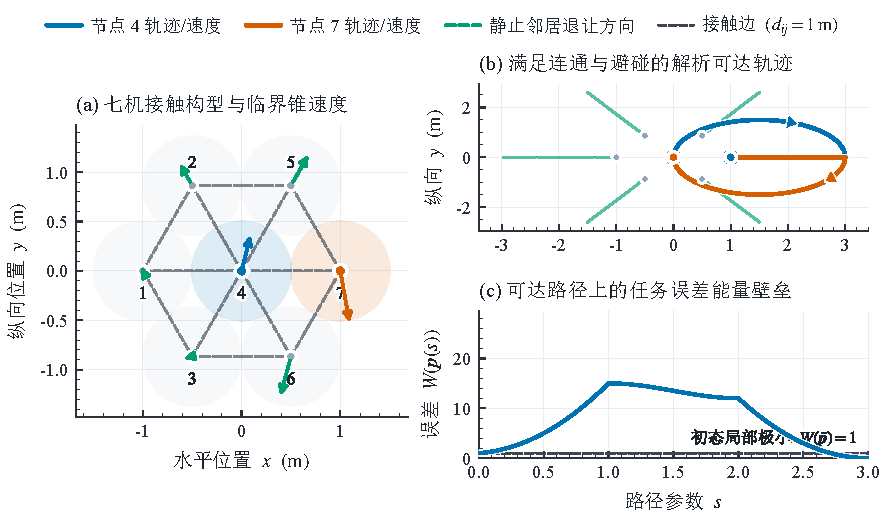
\includegraphics[width=\textwidth]{figures_zh/fig1_seven_geometry.pdf}
 \caption[七机器人严格局部极小构型与安全可达路径构造]{七机器人严格非目标局部极小构型与安全可达路径构造。(a) 式\eqref{eq:seven-config}的双三角对称接触构型、12 条初始接触边与式\eqref{eq:certificate-primal}的临界锥最优速度见证向量；(b) 先均匀放大 $3$ 倍、节点 $4$ 与 $7$ 沿相反半圆交换位置、再均匀缩回的解析安全可达轨迹；(c) 沿可达路径的任务误差曲线 $W(\bp(s))$（任何安全可达轨迹必须先越过高于初态 $W(\bar\bp)=1$ 的能量壁垒）。}
 \label{fig:seven-geom}
\end{figure*}

\begin{theorem}[七机器人对称接触构型的严格局部极小有理数证书与能量壁垒]\label{thm:seven-kkt}
对于式\eqref{eq:seven-config}定义的七机器人位置互换任务（$\ds=1\ \mathrm m,\lr=5/2,R_c=10\ \mathrm m$），成立如下精确结论：
\begin{enumerate}
 \item \textbf{一阶平稳性与二阶临界锥严格正定性：} 在初态 $\bar\bp$ 处，$W(\bar\bp)=1$，$\lambda_2(\bL(\bar\bp))>5/2$，且 $\nabla W(\bar\bp)=\frac12\nabla h_{47}^{\mathrm{col}}(\bar\bp)$，故 $\bu_G=\boldsymbol 0$ 为式\eqref{eq:central-proj}的精确最优解。记完整临界方向锥为 $\mathcal C=\{\boldsymbol v\in\mathbb R^{14}:\bar\bp_{ij}^{\top}(\boldsymbol v_i-\boldsymbol v_j)\ge 0\ (\forall\{i,j\}\in\mathcal E_c),\ v_{4x}=v_{7x}\}$，拉格朗日 Hessian 为 $\boldsymbol H_L=\I_{14}-(\boldsymbol b_{47}\boldsymbol b_{47}^{\top})\otimes\I_2$，则在 $\mathcal C$ 上恒有精确有理数下界
 \begin{equation}
\begin{split}
  \min_{\boldsymbol v\in\mathcal C,\ v_{4y}-v_{7y}=1}\norm{\boldsymbol v}_2^2&=\frac{515}{496}>1,\\
  \boldsymbol v^{\top}\boldsymbol H_L\boldsymbol v&\ge\frac{19}{515}\norm{\boldsymbol v}_2^2>0\quad(\forall\boldsymbol v\in\mathcal C\setminus\{\boldsymbol 0\}).
\end{split}
  \label{eq:critical-hessian}
 \end{equation}
 \item \textbf{有限邻域球面二次能量壁垒与严格内部开球陷阱：} 对任意满足全部机间避碰约束（$d_{ij}(\bar\bp+\boldsymbol\delta)\ge 1$）的非零位置扰动 $0<\norm{\boldsymbol\delta}_2\le\frac1{200}$，恒有显式能量上升下界
 \begin{equation}
  W(\bar\bp+\boldsymbol\delta)-W(\bar\bp)\ge\frac{1}{100}\norm{\boldsymbol\delta}_2^2>0.
  \label{eq:finite-barrier}
 \end{equation}
 进一步，对初态与目标均严格位于安全集内部（无初始接触）的微扰任务 $\bp_0=(1+10^{-8})\bar\bp,\bg_\tau=(1+10^{-6})\bg$，以 $\bp_0$ 为中心、半径 $\rho=\frac1{4\times 10^8}$ 的开球 $B_\rho(\bp_0)\subset\operatorname{int}(\mathcal S)$ 内任一初态出发的连续安全轨迹，若满足 $\dot W_\tau\le 0$，则永远被困于球面 $\norm{\bp-\bar\bp}_2=\frac1{200}$ 内部（球面壁垒 $W_\tau(\bar\bp+\boldsymbol\delta)-W_\tau(\bar\bp)\ge\frac{19}{8\times 10^7}>W_\tau(\bp)-W_\tau(\bar\bp)$），无法到达球外目标 $\bg_\tau$。
 \item \textbf{全局安全与谱连通可达性：} 存在一条显式连续分段光滑路径 $\bp(s)\ (s\in[0,3])$ 连接初态与目标，全程严格满足避碰距离 $d_{ij}(s)\ge 1\ \mathrm m$ 以及代数连通度下界 $\lambda_2(\bL(\bp(s)))\ge\frac{1792}{625}=2.8672>\frac52$。
\end{enumerate}
\end{theorem}
\begin{proof}
（1）在 $\bar\bp$ 处，$\be_4=(-1,0)^{\top},\be_7=(1,0)^{\top}$，其余 $\be_i=\boldsymbol 0$；接触边 $\{4,7\}$ 的障碍梯度在节点 $4,7$ 分量上分别为 $2(\bar\bp_4-\bar\bp_7)=(-2,0)^{\top}$ 与 $2(\bar\bp_7-\bar\bp_4)=(2,0)^{\top}$，故取乘子 $\lambda_{47}=\frac12$、其余乘子为 $0$ 即满足平稳性 $\nabla W(\bar\bp)-\frac12\nabla h_{47}^{\mathrm{col}}(\bar\bp)=\boldsymbol 0$。沿临界方向 $\boldsymbol v\in\mathcal C$，因 $v_{4x}=v_{7x}$，有 $\boldsymbol v^{\top}\boldsymbol H_L\boldsymbol v=\norm{\boldsymbol v}_2^2-|v_{4y}-v_{7y}|^2$。将速度按有理数坐标缩放表示为 $\boldsymbol v_i=(z_{ix},\sqrt{3}z_{iy})^{\top}$ 并堆叠为 $\boldsymbol z\in\mathbb R^{14}$，令对角矩阵 $Q_c=\diag(1,3,\dots,1,3)$，则 $\norm{\boldsymbol v}_2^2=\boldsymbol z^{\top}Q_c\boldsymbol z$。定义有理数接触矩阵 $(G_c\boldsymbol z)_{ij}=\bar p_{ij,x}(z_{ix}-z_{jx})+\sqrt{3}\bar p_{ij,y}(z_{iy}-z_{jy})$ 与等式矩阵 $E_c\boldsymbol z=[z_{4x}-z_{7x},\,z_{4y}-z_{7y}]^{\top}$，考察凸二次规划 $\min\boldsymbol z^{\top}Q_c\boldsymbol z\ \text{s.t.}\ G_c\boldsymbol z\ge\boldsymbol 0,\,E_c\boldsymbol z=(0,1)^{\top}$。构造精确有理数原始解见证 $Z_*\in\mathbb Q^{7\times 2}$ 与对偶乘子 $(\boldsymbol\mu,\boldsymbol\nu)$：
\begin{equation}
\begin{split}
 Z_*^{\top}&=\frac{1}{496}{\setlength{\arraycolsep}{2.5pt}\begin{bmatrix}
 -15 & -132 & -105 & 90 & 177 & -105 & 90\\
 15 & 132 & -15 & 206 & 177 & -225 & -290
 \end{bmatrix}},\\
 \mu_{13}&=\tfrac{15}{248},\ \mu_{24}=\tfrac{33}{62},\ \mu_{36}=\tfrac{15}{62},\ \mu_{45}=\tfrac{177}{248},\ \mu_{67}=\tfrac{225}{248},\\
 \boldsymbol\nu&=\big[\tfrac{135}{496},\,\tfrac{1545}{496}\big]^{\top},
\end{split}\label{eq:certificate-primal}
\end{equation}
其余接触边乘子为 $0$。直接由有理数算术核验可知，$\boldsymbol z_*=\col((Z_*)_{1,:}^{\top},\dots,(Z_*)_{7,:}^{\top})$ 满足原始可行性 $G_c\boldsymbol z_*\ge\boldsymbol 0,E_c\boldsymbol z_*=(0,1)^{\top}$、互补松弛 $\boldsymbol\mu^{\top}G_c\boldsymbol z_*=0$ 及平稳性条件 $Q_c\boldsymbol z_*=G_c^{\top}\boldsymbol\mu+E_c^{\top}\boldsymbol\nu$，最优值为 $\boldsymbol z_*^{\top}Q_c\boldsymbol z_*=\frac{1545}{496}$。由凸二次规划强对偶性并除以纵向缩放因子 $(\sqrt{3})^2=3$，即得 $\min_{\boldsymbol v\in\mathcal C,v_{4y}-v_{7y}=1}\norm{\boldsymbol v}_2^2=\frac{1545}{3\times 496}=\frac{515}{496}>1$（由上下反射对称性对 $v_{4y}-v_{7y}=-1$ 同样成立），从而按齐次性得 $\boldsymbol v^{\top}\boldsymbol H_L\boldsymbol v\ge(1-\frac{496}{515})\norm{\boldsymbol v}_2^2=\frac{19}{515}\norm{\boldsymbol v}_2^2$，即式\eqref{eq:critical-hessian}。

（2）设 $\boldsymbol\delta\in\mathbb R^{14}$ 满足 $0<R:=\norm{\boldsymbol\delta}_2\le\frac1{200}$ 及避碰条件 $\norm{\bar\bp_{ij}+\boldsymbol\delta_i-\boldsymbol\delta_j}_2^2\ge 1\ (\forall\{i,j\}\in\mathcal E_c)$。记 $z=\delta_{4x}-\delta_{7x},t=\delta_{4y}-\delta_{7y}$，则 $W(\bar\bp+\boldsymbol\delta)-W(\bar\bp)=\frac12 R^2-z$。若 $z\le 0$，式\eqref{eq:finite-barrier}显然成立；下设 $z>0$。每条接触边的非线性避碰条件展开为 $\bar\bp_{ij}^{\top}(\boldsymbol\delta_i-\boldsymbol\delta_j)\ge -\frac12\norm{\boldsymbol\delta_i-\boldsymbol\delta_j}_2^2\ge -R^2$。将有理缩放坐标下的平稳性恒等式 $Q_c\boldsymbol z_*=G_c^{\top}\boldsymbol\mu+E_c^{\top}\boldsymbol\nu$ 与缩放扰动 $\tilde{\boldsymbol\delta}$ 作内积，利用 $\boldsymbol\mu\ge\boldsymbol 0$、$\sum_{\{i,j\}\in\mathcal E_c}\mu_{ij}=\frac{609}{248}=:S$、$c=\frac{1545}{496}$ 及 Cauchy–Schwarz 不等式，可得 $\frac{c}{\sqrt{3}}|t|\le\sqrt{c}R+SR^2$。因 $S/\sqrt{c}\le\frac32$，平方整理得 $t^2\le\frac{496}{515}R^2(1+\frac32 R)^2$。又由交换边 $\{4,7\}$ 的避碰条件 $(-1+z)^2+t^2\ge 1\implies 2z\le z^2+t^2$，结合 $z\le\sqrt{2}R<1$ 与 $t^2\le 2R^2$ 可得 $z\le 2R^2$，代入 $2z\le z^2+t^2$ 得 $z\le 2R^4+\frac12 t^2$。因此
\begin{equation}
\begin{split}
 W(\bar\bp+\boldsymbol\delta)-W(\bar\bp)&=\frac12 R^2-z\\
 &\ge\frac{R^2}{2}\left[1-\frac{496}{515}\Big(1+\frac32 R\Big)^2-4R^2\right]\\
 &\ge\frac{1}{100}R^2,\qquad\forall R\in\Big(0,\frac1{200}\Big].
\end{split}
\end{equation}
对于严格内部微扰版本 $\bp_0=(1+10^{-8})\bar\bp,\bg_\tau=(1+10^{-6})\bg$，在球面 $\norm{\boldsymbol\delta}_2=r=\frac1{200}$ 上由 $\norm{\bg}_2=\sqrt{6}<\frac52$ 得 $W_\tau(\bar\bp+\boldsymbol\delta)-W_\tau(\bar\bp)=W(\bar\bp+\boldsymbol\delta)-W(\bar\bp)-\tau\bg^{\top}\boldsymbol\delta\ge\frac{r^2}{100}-\frac52\tau r=\frac{19}{8\times 10^7}$，而在开球 $B_\rho(\bp_0)$ 内最大误差增量严格低于该球面壁垒，故任何单调不增的安全轨迹均无法穿过球面 $\norm{\bp-\bar\bp}_2=\frac1{200}$。

（3）构造图\ref{fig:seven-geom}(b) 所示的三阶段路径：$s\in[0,1]$ 时全体位置均匀放大至 $3\bar\bp$；$s\in[1,2]$ 时外围五机保持在 $3\bar\bp_i$，节点 $4$ 与 $7$ 绕中心 $(3/2,0)$ 沿半径 $3/2$ 的相反半圆交换位置；$s\in[2,3]$ 时全体位置从 $3\bg$ 均匀缩回 $\bg$。在半圆交换阶段，节点 $4,7$ 间距恒为 $3\ge 1$，外围五机到圆心 $(3/2,0)$ 的距离平方最小为 $\frac{27}{4}>(\frac32+1)^2=\frac{25}{4}$，故全程满足 $d_{ij}(s)\ge 1$。全程任意两机最大距离不超过 $6\ \mathrm m$，由式\eqref{eq:poly-channel}知每条完全图边权满足 $w_{ij}(s)\ge(1-\frac{36}{100})^2=\frac{256}{625}$，故 $\lambda_2(\bL(\bp(s)))\ge 7\times\frac{256}{625}=\frac{1792}{625}>\frac52$。
\end{proof}

\begin{remark}[七机器人见证启发的协同控制构造]\label{rem:two-conditions}
定理\ref{thm:seven-kkt}及见证式\eqref{eq:certificate-primal}启发以下两项控制构造。它们描述本文采用的局部脱困机制，不构成任意重排任务的全局充要条件：
\begin{enumerate}
 \item \textbf{待互换机器人的侧向破对称标称驱动：} 在临界锥最优错开方向式\eqref{eq:certificate-primal}中，中心机器人 $4$ 与右侧机器人 $7$ 必须产生相反的纵向（垂直于目标误差 $\be_4,\be_7$）速度分量 $z_{4y}=+\frac{206}{496}>0$ 与 $z_{7y}=-\frac{290}{496}<0$（图\ref{fig:seven-geom}(a) 蓝色与橙色箭头）。若标称控制器仅提供沿 $\be_i$ 方向的径向吸引，则系统永远停留在 $v_{4y}-v_{7y}=0$ 的共线死锁子空间内。
 \item \textbf{外围静止邻居经由动态配额让渡实现的协同退让：} 式\eqref{eq:certificate-primal}表明，当机器人 $4$ 与 $7$ 沿纵向错开时，周围五台原本已处于各自目标位置（$\be_j=\boldsymbol 0$）的静止邻居必须同步产生非零向外退让速度（如 $(Z_*)_{2,:}=\frac1{496}[-132,132]$、$(Z_*)_{5,:}=\frac1{496}[177,177]$，见图\ref{fig:seven-geom}(a) 翠绿色箭头），该运动通过接触边上的严格正对偶乘子 $\mu_{24},\mu_{45},\mu_{67}>0$ 实现力学传递。若安全滤波器采用静态配额平摊（固定各节点在避碰行上的份额为零），则 $\be_j=\boldsymbol 0$ 的静止邻居保持 $\bu_j=\boldsymbol 0$，接触约束直接把机器人 $4$ 与 $7$ 的纵向错开分量截断为零。
\end{enumerate}
上述两项机理直接决定了第\ref{sec:method}节的 EGP-NPA 控制架构设计：由等变图网络强化学习策略为受阻移动机器人提供手性侧向绕行标称速度，并由闭邻域块 NPA 滤波器的动态零和份额转移驱动外围静止邻居协同退让。
\end{remark}

\section{包络等变图策略与邻域近端分配协同控制（EGP-NPA）}\label{sec:method}

\subsection{手性旋转与置换等变的图神经网络残差标称架构}\label{subsec:gnn-arch}
为在不依赖人工构造全局拓扑势函数的前提下打破注\ref{rem:two-conditions}指出的共线死锁，在采样时刻 $t_k=k\Delta t$、感知与通信半径 $R_{\mathrm{sense}}=2.50\ \mathrm m$ 定义的一跳有向通信图 $\mathcal G_{\mathrm c}(\bp_k)=(\mathcal V,\mathcal E_k)$ 上构建分布式残差标称策略。

直接将笛卡尔坐标 $\bp_{i,k},\bg_i$ 输入神经网络会破坏欧氏空间的刚体变换不变性，导致同一相对队形在旋转或平移至不同工作区位置时产生不一致的策略输出，降低样本效率并损害跨规模泛化能力\cite{satorras2021egnn}。为此，对每个机器人 $i\in\mathcal V$，以其单位目标误差方向 $\hat{\be}_{i,k}=\be_{i,k}/\max(\norm{\be_{i,k}}_2,10^{-9})$ 与逆时针正交旋转 $90^\circ$ 向量 $\bJ\hat{\be}_{i,k}$ 张成局部目标参考标架；对每条有向通信边 $(i,j)\in\mathcal E_k$，以单位相对位置向量 $\hat{\br}_{ij,k}=(\bp_{j,k}-\bp_{i,k})/d_{ij,k}$ 与 $\bJ\hat{\br}_{ij,k}$ 张成局部边参考标架，并引入目标平滑消隐因子 $\sigma_{i,k}=\min(1,\norm{\be_{i,k}}_2/r_0)$（取 $r_0=0.10\ \mathrm m$）以消除 $\be_{i,k}\to\boldsymbol 0$ 时的方向角奇异性。

记节点 $i$ 上一拍实际执行速度为 $\bu_{i,k-1}$，经速度球裁剪后的标称参考与实际执行速度之差（即滤波器速度修正量）为 $\boldsymbol\delta_{i,k-1}=\bu_{i,k-1}-\Pi_{\mathcal U_i}(\bu_{i,k-1}^{\mathrm{nom}})$，上一拍单机安全重拟合式\eqref{eq:refit-one}的非负拉格朗日对偶乘子（碰撞与谱影子价格）为 $\boldsymbol\mu_{i,k-1}$，谱约束分配配额为 $s_{i0,k-1}$，边 $e=\{i,j\}$ 上的二元边记录为 $\boldsymbol\varpi_{e,k-1}=[\varpi_{ij,0,k-1},\varpi_{ij,1,k-1}]^{\top}$。定义一跳闭邻域冲突记忆状态 $m_{i,k}=\max\bigl(\gamma_m m_{i,k-1},\max_{j\in\mathcal N_{i,k}^+}c_{j,k-1}\bigr)$ 及其冲突记忆门控因子 $\gamma_{i,k}^{\mathrm{gate}}=\tanh(\beta_m m_{i,k})\in[0,1)$（其中记忆衰减率 $\gamma_m=0.97$，增益 $\beta_m=4.0$；取 $c_{j,k-1}=\norm{\boldsymbol\mu_{j,k-1}}_2$ 对应影子价格门控 $\gamma_{i,k}^{\mathrm{gate},\mu}$，取 $c_{j,k-1}=\norm{\boldsymbol\delta_{j,k-1}}_2$ 对应滤波修正量门控 $\gamma_{i,k}^{\mathrm{gate,int}}$）。节点 $i$ 的旋转不变特征 $\boldsymbol x_{i,k}=\col(\boldsymbol x_{i,k}^{\mathrm{geom}},\boldsymbol x_{i,k}^{\mathrm{alg}})\in\mathbb R^{17}$ 与有向边 $(i,j)$ 的旋转不变特征 $\boldsymbol e_{ij,k}^{\mathrm{feat}}=\col(\boldsymbol e_{ij,k}^{\mathrm{geom}},\boldsymbol e_{ij,k}^{\mathrm{alg}})\in\mathbb R^{20}$ 由几何投影子向量与滤波器内部代数状态经对数/双曲正切压缩构成：
\begin{equation}
\begin{split}
 \boldsymbol x_{i,k}^{\mathrm{geom}}&=\Big[\min(\norm{\be_{i,k}}_2,4),\ \mathbb I(\norm{\be_{i,k}}_2<\varepsilon_g),\ \gamma_{i,k}^{\mathrm{gate}},\\
 &\quad\ \tfrac{\norm{\bu_{i,k-1}}_2}{U},\ \tfrac{\bu_{i,k-1}^{\top}\hat{\be}_{i,k}}{U}\sigma_{i,k},\ \tfrac{\bu_{i,k-1}^{\top}\bJ\hat{\be}_{i,k}}{U}\sigma_{i,k},\\
 &\quad\ \tfrac{\norm{\boldsymbol\delta_{i,k-1}}_2}{U},\ \tfrac{\boldsymbol\delta_{i,k-1}^{\top}\hat{\be}_{i,k}}{U}\sigma_{i,k},\ \tfrac{\boldsymbol\delta_{i,k-1}^{\top}\bJ\hat{\be}_{i,k}}{U}\sigma_{i,k},\\
 &\quad\ \tfrac{\lambda_2(\bL(\bp_k))-\lr}{\lr},\ \tfrac{|\mathcal N_{i,k}|}{8},\ \min_{j\in\mathcal N_{i,k}}(d_{ij,k}-\ds)\Big]^{\top},
\end{split}\label{eq:node-geom}
\end{equation}
\begin{equation}
\begin{split}
 \boldsymbol e_{ij,k}^{\mathrm{geom}}&=\Big[\tfrac{d_{ij,k}}{R_{\mathrm{sense}}},\ \clip(d_{ij,k}-\ds,0,1.5),\ \hat{\br}_{ij,k}^{\top}\hat{\be}_{i,k}\sigma_{i,k},\\
 &\quad\ \hat{\br}_{ij,k}^{\top}\bJ\hat{\be}_{i,k}\sigma_{i,k},\ \hat{\br}_{ij,k}^{\top}\hat{\be}_{j,k}\sigma_{j,k},\ \hat{\br}_{ij,k}^{\top}\bJ\hat{\be}_{j,k}\sigma_{j,k},\\
 &\quad\ \min(\norm{\be_{j,k}}_2,4),\ \hat{\be}_{i,k}^{\top}\hat{\be}_{j,k}\sigma_{i,k}\sigma_{j,k},\\
 &\quad\ (\bJ\hat{\be}_{i,k})^{\top}\hat{\be}_{j,k}\sigma_{i,k}\sigma_{j,k},\ \tfrac{(\bu_{j,k-1}-\bu_{i,k-1})^{\top}\hat{\br}_{ij,k}}{U},\\
 &\quad\ \tfrac{(\bu_{j,k-1}-\bu_{i,k-1})^{\top}\bJ\hat{\br}_{ij,k}}{U},\ \gamma_{j,k}^{\mathrm{gate}},\ \tfrac{\norm{\boldsymbol\delta_{j,k-1}}_2}{U}\Big]^{\top},
\end{split}\label{eq:edge-geom}
\end{equation}
\begin{equation}
\begin{split}
 \boldsymbol x_{i,k}^{\mathrm{alg}}&=\Big[\ln(1+|\mu_{i0,k-1}|),\ \ln\big(1+\textstyle\sum_{j\ne i}|\mu_{ij,k-1}|\big),\\
 &\quad\ \clip\big(\tfrac{s_{i0,k-1}}{\bar\nu_{i0,k}},-3,3\big),\ \ln(1+\norm{\boldsymbol\mu_{i,k-1}}_2),\\
 &\quad\ \clip\big(\tfrac{U\norm{\boldsymbol a_{i0,k}}_2-b_{i0,k}-s_{i0,k-1}}{\bar\nu_{i0,k}},-3,3\big)\Big]^{\top},\\
 \boldsymbol e_{ij,k}^{\mathrm{alg}}&=\Big[\ln(1+|\mu_{ij,k-1}|),\ \ln(1+|\mu_{ji,k-1}|),\\
 &\quad\ \tanh(2\varpi_{ij,0,k-1}),\ \tanh(2\varpi_{ij,1,k-1}),\\
 &\quad\ |\tilde\phi_{i,k}-\tilde\phi_{j,k}|,\ \norm{\widetilde{\boldsymbol\Phi}_{i,k}-\widetilde{\boldsymbol\Phi}_{j,k}}_2,\ \widetilde{\boldsymbol\Phi}_{i,k}^{\top}\widetilde{\boldsymbol\Phi}_{j,k}\Big]^{\top},
\end{split}\label{eq:alg-feat}
\end{equation}
其中 $\bar\nu_{i0,k}=U\norm{\boldsymbol a_{i0,k}}_2+|b_{i0,k}|+10^{-3}$ 为全局标量约束行归一化尺度，$\tilde\phi_{i,k}=\sqrt{N}\phi_{i,k}$ 与 $\widetilde{\boldsymbol\Phi}_{i,k}=\sqrt{N}\boldsymbol\Phi_{i,k}\in\mathbb R^2$ 分别为按单位均方幅值约定（满足 $\frac1N\sum_{i=1}^N\tilde\phi_{i,k}^2=1$）的无量纲标量拉普拉斯谱坐标，使各节点仅通过本地差分与内积即可表征与全网规模 $N$ 无关的拓扑相对位置。式\eqref{eq:node-geom}--\eqref{eq:alg-feat}中所有二维几何向量均通过局部正交标架内积化为刚体不变标量；代数子向量 $\boldsymbol x_{i,k}^{\mathrm{alg}},\boldsymbol e_{ij,k}^{\mathrm{alg}}$ 则向策略网络显式暴露各接触边的紧迫度影子价格 $\mu_{ij,k-1}$ 与配额储备状态。

参数共享的 $L_{\mathrm{gnn}}=2$ 层消息传递图网络首先将节点特征编码为 $\boldsymbol h_i^{(0)}=\phi_{\mathrm{enc}}(\boldsymbol x_{i,k})\in\mathbb R^{d_h}$（隐层维数 $d_h=64$），随后在每层 $\ell\in\{1,\dots,L_{\mathrm{gnn}}\}$ 执行一跳消息计算与均值—最大值双聚合更新（其中均值聚合捕获邻域整体拥挤趋势，逐分量最大值聚合保留最紧迫的单个接触阻挡邻居特征）：
\begin{equation}
\begin{split}
 \boldsymbol m_{ij}^{(\ell)}&=\phi_{\mathrm{msg}}^{(\ell)}\big(\col(\boldsymbol h_i^{(\ell-1)},\boldsymbol h_j^{(\ell-1)},\boldsymbol e_{ij,k}^{\mathrm{feat}})\big),\quad\forall (i,j)\in\mathcal E_k,\\
 \bar{\boldsymbol m}_i^{(\ell)}&=\frac{1}{\max(|\mathcal N_{i,k}|,1)}\sum_{j\in\mathcal N_{i,k}}\boldsymbol m_{ij}^{(\ell)},\quad
 \hat{\boldsymbol m}_i^{(\ell)}=\max_{j\in\mathcal N_{i,k}}\boldsymbol m_{ij}^{(\ell)},\\
 \boldsymbol h_i^{(\ell)}&=\operatorname{LN}^{(\ell)}\!\Big(\boldsymbol h_i^{(\ell-1)}+\phi_{\mathrm{upd}}^{(\ell)}\big(\col(\boldsymbol h_i^{(\ell-1)},\bar{\boldsymbol m}_i^{(\ell)},\hat{\boldsymbol m}_i^{(\ell)})\big)\Big),
\end{split}\label{eq:gnn-layer}
\end{equation}
式中 $\phi_{\mathrm{enc}},\phi_{\mathrm{msg}}^{(\ell)},\phi_{\mathrm{upd}}^{(\ell)}$ 为采用 $\operatorname{SiLU}$ 激活函数的多层感知机（MLP），$\operatorname{LN}^{(\ell)}$ 为层归一化（Layer Normalization）算子。经 $L_{\mathrm{gnn}}$ 层传播后，节点输出头 $\phi_{\mathrm{node}}$ 与边输出头 $\phi_{\mathrm{edge}}$ 生成三个有界标量动作系数：
\begin{equation}
\begin{split}
 (\omega_{i,k}^\theta,r_{i,k}^\theta)&=\clip\big(\phi_{\mathrm{node}}(\boldsymbol h_i^{(L_{\mathrm{gnn}})}),-1,1\big),\\
 \psi_{ij,k}^\theta&=\clip\big(\phi_{\mathrm{edge}}(\col(\boldsymbol h_i^{(L_{\mathrm{gnn}})},\boldsymbol h_j^{(L_{\mathrm{gnn}})},\boldsymbol e_{ij,k}^{\mathrm{feat}})),-1,1\big),
\end{split}
 \label{eq:action-heads}
\end{equation}
并在局部正交基上合成为机器人 $i$ 的二维标称参考速度：
\begin{equation}
\begin{split}
 \bu_{i,k}^{\mathrm{nom}}(\bp_k;\theta)&=-\be_{i,k}+\gamma_{i,k}^{\mathrm{eff}}\br_{i,k}^\theta(\bp_k),\\
 \br_{i,k}^\theta(\bp_k)&=A_{\mathrm{rot}}\omega_{i,k}^\theta\bJ\be_{i,k}+A_{\mathrm{rad}}r_{i,k}^\theta\be_{i,k}\\
 &\quad+\frac{A_\psi U}{\max(|\mathcal N_{i,k}|,1)}\sum_{j\in\mathcal N_{i,k}}\psi_{ij,k}^\theta\frac{\bp_{i,k}-\bp_{j,k}}{d_{ij,k}},
\end{split}\label{eq:nominal-law}
\end{equation}
其中 $\gamma_{i,k}^{\mathrm{eff}}\in[0,1)$ 为综合包络门控因子（定义见第\ref{subsec:envelope}节），幅值增益取 $A_{\mathrm{rot}}=2.0\ \mathrm s^{-1},A_{\mathrm{rad}}=1.5\ \mathrm s^{-1},A_\psi=2.0$。式\eqref{eq:nominal-law}各项具有清晰的几何分工：$-\be_{i,k}$ 为基础目标吸引项；$A_{\mathrm{rot}}\omega_{i,k}^\theta\bJ\be_{i,k}$ 为垂直于目标视线的切向环流项，负责在迎头交会时驱动移动节点向侧面斜插绕行以打破共线对称平衡；$A_{\mathrm{rad}}r_{i,k}^\theta\be_{i,k}$ 为径向伸缩项，调节接近目标的推进速率；$\sum_{j\in\mathcal N_{i,k}}\psi_{ij,k}^\theta(\bp_{i,k}-\bp_{j,k})/d_{ij,k}$ 为沿一跳邻居连线方向的成对避让偏置项。

\begin{proposition}[标称控制场的平面刚体变换与置换等变性及手性破缺机理]\label{prop:equivariance}
对任意网络参数 $\theta$、任意平面旋转矩阵 $\boldsymbol R\in\mathrm{SO}(2)$、平移向量 $\boldsymbol c\in\mathbb R^2$ 以及任意 $N\times N$ 节点置换矩阵 $\boldsymbol P_\pi$，令刚体变换同步作用于全体节点位置、目标与历史速度（$\tilde\bp_i=\boldsymbol R\bp_i+\boldsymbol c,\tilde\bg_i=\boldsymbol R\bg_i+\boldsymbol c,\tilde\bu_{i,k-1}=\boldsymbol R\bu_{i,k-1}$），则式\eqref{eq:nominal-law}定义的标称控制场满足旋转平移等变性与节点置换等变性：
\begin{equation}
\begin{split}
 \bu_{i,k}^{\mathrm{nom}}(\tilde\bp_k,\tilde\bg;\theta)&=\boldsymbol R\bu_{i,k}^{\mathrm{nom}}(\bp_k,\bg;\theta),\\
 \bu_k^{\mathrm{nom}}\big((\boldsymbol P_\pi\otimes\I_2)\bp_k,(\boldsymbol P_\pi\otimes\I_2)\bg\big)&=(\boldsymbol P_\pi\otimes\I_2)\bu_k^{\mathrm{nom}}(\bp_k,\bg).
\end{split}\label{eq:equiv-prop}
\end{equation}
进一步，若将式\eqref{eq:nominal-law}强制约束为全正交群 $\mathrm{O}(2)$（含平面镜像反射 $\boldsymbol M\in\mathrm{O}(2)\setminus\mathrm{SO}(2),\det\boldsymbol M=-1$）等变，则在任意关于各自目标视线轴镜像对称的迎头交会构型上，切向破对称系数必然退化为 $\omega_{i,k}^\theta\equiv 0$。
\end{proposition}
\begin{proof}
在刚体变换下，相对位移满足 $\tilde\be_{i,k}=\boldsymbol R\be_{i,k}$ 与 $\tilde\bp_{i,k}-\tilde\bp_{j,k}=\boldsymbol R(\bp_{i,k}-\bp_{j,k})$，平移向量 $\boldsymbol c$ 完全抵消。由于 $\boldsymbol R\in\mathrm{SO}(2)$ 保范数、保内积且与二维反对称旋转算子 $\bJ$ 满足可交换性 $\boldsymbol R\bJ=\bJ\boldsymbol R$，式\eqref{eq:node-geom}--\eqref{eq:alg-feat}中的全部内积项（如 $(\boldsymbol R\bu_{i,k-1})^{\top}(\boldsymbol R\bJ\hat{\be}_{i,k})=\bu_{i,k-1}^{\top}\bJ\hat{\be}_{i,k}$）及拉普拉斯谱量均严格保持不变，故标量动作系数满足 $(\tilde\omega_{i,k}^\theta,\tilde r_{i,k}^\theta,\tilde\psi_{ij,k}^\theta)=(\omega_{i,k}^\theta,r_{i,k}^\theta,\psi_{ij,k}^\theta)$。将其代入式\eqref{eq:nominal-law}并再次利用 $\boldsymbol R\bJ\be_{i,k}=\bJ\boldsymbol R\be_{i,k}$ 即得第一式；节点置换等变性由消息传递式\eqref{eq:gnn-layer}对全体节点与有向边共享网络参数及均值/最大值聚合算子的置换不变性直接推出。反之，对任意平面镜像反射矩阵 $\boldsymbol M\in\mathrm{O}(2)\setminus\mathrm{SO}(2)$（$\det\boldsymbol M=-1$），恒有反对易关系 $\boldsymbol M\bJ=-\bJ\boldsymbol M$。若构型与历史状态关于节点 $i$ 的目标误差轴 $\hat{\be}_{i,k}$ 镜像对称（即 $\boldsymbol M\be_{i,k}=\be_{i,k}$ 且邻域构型满足 $\boldsymbol M$ 对称不变），则 $\mathrm{O}(2)$ 等变性要求 $\boldsymbol M\bu_{i,k}^{\mathrm{nom}}=\bu_{i,k}^{\mathrm{nom}}$，在正交方向 $\bJ\be_{i,k}$ 上投影即给出 $-\omega_{i,k}^\theta=\omega_{i,k}^\theta\implies\omega_{i,k}^\theta\equiv 0$。
\end{proof}

命题\ref{prop:equivariance}从群表示论角度揭示了破除对称死锁的一条关键设计准则：标称策略必须设计为特殊正交群 $\mathrm{SO}(2)$ 等变而非 $\mathrm{O}(2)$ 镜像等变，通过保留确定性的手性旋转偏置（Chirality），使受阻机器人在完全对称的迎头平衡点处能够一致地选择同一手性方向斜插绕行。

\subsection{闭邻域动态分摊护盾与外围静止邻居协同退让机理}\label{subsec:npa-yield}
各机器人由式\eqref{eq:nominal-law}生成标称参考速度 $\bu_{i,k}^{\mathrm{nom}}$ 后，送入第\ref{subsec:npa-prelim}节的闭邻域近端分配（NPA）及边记录本地结清安全滤波器 $L$（每拍执行 $B$ 轮局部协商）求解实际执行速度 $\bu_{i,k}$，并在零阶保持执行前经过定理\ref{thm:zoh-safe}的精确有理数整段安全证书核验。

\begin{proposition}[学习探索与有限轮跨规模执行的随时硬安全不变性]\label{prop:safety}
设初态满足 $\bp_0\in\mathcal S$，耦合安全约束满足零速可行初值条件 $b_{ia,k}\le 0$。则无论图网络策略参数 $\theta$ 如何取值（含训练初期叠加高斯探索噪声的随机策略及任意跨规模 $N$ 的零样本部署），也无论每拍分配轮数 $B\ge 0$ 是否收敛至全局集中式最优解，经闭邻域动态分摊护盾 $L$ 与零阶保持精确有理数证书执行后的闭环轨迹在全部连续时间 $t\ge 0$ 上恒满足机间避碰 $d_{ij}(t)\ge\ds\ (\forall i<j)$、全局代数连通度下界 $\lambda_2(\bL(\bp(t)))\ge\lr$ 以及输入幅值与工作区约束。
\end{proposition}
\begin{proof}
由式\eqref{eq:edge-ledger}的反对称边记录结构，在任意采样时刻 $t_k$，经阶段一断边撤销与一跳本地结清后，初始配额 $\boldsymbol s_k^{(0)}$ 恒满足全局零和条件 $\sum_{i\in\mathcal V_a}s_{ia,k}^{(0)}=0$ 且热启动速度 $\bu_k^{(0)}$ 满足单机约束式\eqref{eq:refit-one}。在阶段二的任意第 $r\in\{1,\dots,B\}$ 轮，每个闭邻域块二次规划式\eqref{eq:block-qp}的局部增量满足 $\sum_{q\in\mathcal N_{i,k}^+}w_q=0$ 及成对边转移反对称性 $\sigma_{q,e}t_e+\sigma_{m,e}t_e=0$，按式\eqref{eq:convex-commit}作凸组合提交后，迭代解 $(\bu_k^{(B)},\boldsymbol s_k^{(B)})$ 严格保持配额零和性与全网耦合线性化约束式\eqref{eq:coupled-rows}。再结合定理\ref{thm:zoh-safe}的整段步长自适应减半有理数核验，每个采样保持段 $[t_k,t_k+h_k]$ 上的连续轨迹恒位于复合安全集 $\mathcal S$ 内，由归纳法知全时域 $t\ge 0$ 硬安全不变性成立。
\end{proof}

下面从代数上严格证明：为什么闭邻域块二次规划式\eqref{eq:block-qp}中的动态份额转移变量 $t_e$ 是驱动外围静止邻居让出通道的核心机制，而静态配额平摊（$B=0$）会导致机器人人为冻结。

\begin{proposition}[闭邻域动态份额转移对静止阻挡邻居的协同解冻性质]\label{prop:unfreeze}
考察密集格点内部互换中的典型接触单元：待移动机器人 $i$ 与已处于自身目标位置的静止邻居 $j$（$\be_j=\boldsymbol 0$，其自身标称速度为 $\bu_j^{\mathrm{nom}}=\boldsymbol 0$）处于接触边界 $d_{ij}=\ds$（此时碰撞裕度常数项 $b_{ia}=b_{ja}=0$），记从 $j$ 指向 $i$ 的单位接触法向量为 $\boldsymbol n_{ij}=(\bp_i-\bp_j)/\ds$。设图网络残差策略式\eqref{eq:nominal-law}为机器人 $i$ 生成了指向静止邻居 $j$ 方向的非零侧向绕行标称速度（满足法向侵入量 $\delta_n := -\boldsymbol n_{ij}^{\top}\bu_i^{\mathrm{nom}}>0$，且幅值未饱和）：
\begin{enumerate}
 \item \textbf{静态配额平摊（$B=0, s_{ia}=s_{ja}\equiv 0$）下的人为冻结：} 机器人 $i$ 与 $j$ 的局部避碰约束退化为各自独立的半空间约束 $-2\ds\boldsymbol n_{ij}^{\top}\bu_i\le 0$ 与 $2\ds\boldsymbol n_{ij}^{\top}\bu_j\le 0$。由于 $\bu_j^{\mathrm{nom}}=\boldsymbol 0$ 已满足节点 $j$ 的约束，单机投影输出 $\bu_j^{\mathrm{stat}}=\boldsymbol 0$（静止邻居纹丝不动）；而机器人 $i$ 指向 $j$ 的法向速度分量被单机约束强制截断为零（$-\boldsymbol n_{ij}^{\top}\bu_i^{\mathrm{stat}}=0$），侧向绕行通道被完全封死。
 \item \textbf{闭邻域动态分摊（$B\ge 1$）下的份额让渡与协同退让：} 在式\eqref{eq:block-qp}的两节点接触子问题（从零初始份额出发）中，唯一最优解产生的成对避碰份额转移量 $t_{ij}^\star$、移动机器人法向推进速度 $-\boldsymbol n_{ij}^{\top}\bu_i^\star$ 与静止邻居向外退让速度 $-\boldsymbol n_{ij}^{\top}\bu_j^\star$ 具有显式严格正闭式解：
 \begin{equation}
\begin{split}
  |t_{ij}^\star| &= \frac{\eta\ds}{\eta+4\ds^2}\delta_n > 0,\\
  -\boldsymbol n_{ij}^{\top}\bu_i^\star &= -\boldsymbol n_{ij}^{\top}\bu_j^\star = \frac{\eta}{2(\eta+4\ds^2)}\delta_n > 0.
\end{split}
  \label{eq:joint-yield}
 \end{equation}
\end{enumerate}
\end{proposition}
\begin{proof}
在接触边界 $d_{ij}=\ds$ 处，$\boldsymbol a_{ia}=-2\ds\boldsymbol n_{ij},\boldsymbol a_{ja}=2\ds\boldsymbol n_{ij},b_{ia}=b_{ja}=0$。将两节点的速度正交分解为沿 $-\boldsymbol n_{ij}$（即指向 $j$ 外侧的退让方向）的法向标量分量 $u_{q,n}=-\boldsymbol n_{ij}^{\top}\bu_q$ 与切向分量 $\bu_{q,\tau}=(\I_2-\boldsymbol n_{ij}\boldsymbol n_{ij}^{\top})\bu_q$（$q\in\{i,j\}$）。切向分量不受该接触行约束，故 $\bu_{i,\tau}^\star=\bu_{i,\tau}^{\mathrm{nom}},\bu_{j,\tau}^\star=\boldsymbol 0$。对于法向分量：
（1）当 $B=0$ 且 $s_{ia}=s_{ja}=0$ 时，单机约束分别为 $2\ds u_{i,n}\le 0\implies u_{i,n}\le 0$ 与 $-2\ds u_{j,n}\le 0\implies u_{j,n}\ge 0$。因 $u_{i,n}^{\mathrm{nom}}=\delta_n>0,u_{j,n}^{\mathrm{nom}}=0$，各自独立最小化 $\frac12(u_{i,n}-\delta_n)^2$ 与 $\frac12 u_{j,n}^2$ 直接给出 $u_{i,n}^{\mathrm{stat}}=0,u_{j,n}^{\mathrm{stat}}=0$。
（2）在式\eqref{eq:block-qp}的动态分摊块问题中，节点 $i$ 与 $j$ 的法向约束分别为 $2\ds u_{i,n}+t_{ij}\le 0$ 与 $-2\ds u_{j,n}-t_{ij}\le 0$，块目标函数法向部分为 $J_n(u_{i,n},u_{j,n},t_{ij})=\frac12(u_{i,n}-\delta_n)^2+\frac12 u_{j,n}^2+\frac{1}{\eta}t_{ij}^2$。由于 $J_n$ 严格凸且无约束极小点 $(\delta_n,0,0)$ 违反节点 $i$ 的约束（$2\ds\delta_n>0$），由 KKT 互补松弛条件可知两条不等式在最优点处必同时取等号，即 $t_{ij}=-2\ds u_{i,n}=-2\ds u_{j,n}$，从而 $u_{i,n}^\star=u_{j,n}^\star=:v_n$。将其代入 $J_n$ 得单变量严格凸二次函数 $f(v_n)=\frac12(v_n-\delta_n)^2+\frac12 v_n^2+\frac{4\ds^2}{\eta}v_n^2$，求导令 $f'(v_n)=(2+\frac{8\ds^2}{\eta})v_n-\delta_n=0$，解得 $v_n=\frac{\eta}{2(\eta+4\ds^2)}\delta_n>0$ 及 $|t_{ij}^\star|=2\ds v_n=\frac{\eta\ds}{\eta+4\ds^2}\delta_n>0$，即得式\eqref{eq:joint-yield}（在本文标称参数 $\ds=1\ \mathrm m,\eta=2.0$ 下单步系数为 $\frac16$，多轮迭代收敛至集中式投影解 $\delta_n/2$）。
\end{proof}

命题\ref{prop:unfreeze}阐明了强化学习标称层与动态分摊滤波层之间的互补分工：策略网络只需让真正有移动需求的受阻节点 $i$ 学会产生侧向切入分量 $\delta_n>0$，而无需让外围静止邻居在标称层盲目猜测何时离开自身目标点；闭邻域块二次规划通过碰撞份额让渡 $t_{ij}^\star$ 自动将移动节点的侧向绕行意图转化为静止邻居的最小范数退让运动，且一旦移动节点穿过通道（$\delta_n\to 0$），静止邻居立即在 $-\be_j$ 恢复力下归位。同时，式\eqref{eq:joint-yield}表明移动节点 $i$ 在接触法向上的滤波速度修正量为 $u_{i,n}^\star-\delta_n=-\frac{\eta+8\ds^2}{2(\eta+4\ds^2)}\delta_n\ne 0$，即标称速度指向接触边界外侧（$\delta_n>0$）是该接触模型中触发配额转移 $|t_{ij}^\star|>0$ 与邻居协同退让的直接驱动源；若在策略训练损失中惩罚标称指令与滤波安全速度之间的法向偏差以压制 $\delta_n$，则会削弱式\eqref{eq:joint-yield}中的配额让渡与邻居退让速度，其闭环效应将在第\ref{sec:experiments}节中通过主基准与受控析因实验进一步检验。

\subsection{一跳闭邻域终点完成包络与目标平衡点恢复}\label{subsec:envelope}
考察标称控制律式\eqref{eq:nominal-law}在全体机器人趋近目标构型（$\bp_k\to\bg$，即 $\be_{i,k}\to\boldsymbol 0,\ \forall i\in\mathcal V$）时的渐近行为。在式\eqref{eq:nominal-law}的三个残差项中，切向项 $A_{\mathrm{rot}}\omega_{i,k}^\theta\bJ\be_{i,k}$ 与径向项 $A_{\mathrm{rad}}r_{i,k}^\theta\be_{i,k}$ 均显式乘有自身误差向量 $\be_{i,k}$，因而在 $\be_{i,k}\to\boldsymbol 0$ 时自动一阶归零；然而，第三项成对相对避让偏置
\begin{equation}
 \boldsymbol b_{i,k}^\psi := \frac{A_\psi U}{\max(|\mathcal N_{i,k}|,1)}\sum_{j\in\mathcal N_{i,k}}\psi_{ij,k}^\theta\frac{\bp_{i,k}-\bp_{j,k}}{d_{ij,k}}
\end{equation}
是由单位相对方向向量构成的零阶项，其幅值不随 $\be_{i,k}\to\boldsymbol 0$ 自动衰减。在间距 $1.001\ \mathrm m$（仅比安全距离 $\ds=1.000\ \mathrm m$ 大 $1\ \mathrm{mm}$）的密集格点终点处，相邻避碰约束仍处于近激活状态，单机重拟合对偶乘子 $\norm{\boldsymbol\mu_{i,k-1}}_2>0$，导致冲突记忆门控因子 $\gamma_{i,k}^{\mathrm{gate}}=\tanh(\beta_m m_{i,k})$ 在终点附近仍保持 $\gamma_{i,k}^{\mathrm{gate}}\approx 1$。此时非零零阶排斥偏置 $\boldsymbol b_{i,k}^\psi$ 与线性恢复力 $-\be_{i,k}$ 在 $\norm{\be_{i,k}}_2\in[0.015,0.05]\ \mathrm m$ 处形成力平衡或微幅极限环（即终点稳态悬停），阻碍系统进入 $\norm{\be_{i,k}}_2\le 0.01\ \mathrm m$ 的达标判定域。

若仅用节点自身误差 $\tanh(\norm{\be_{i,k}}_2/\varepsilon_g)$ 去乘残差，则初始已处于目标位置的静止邻居（$\be_{i,k}=\boldsymbol 0$）从 $t=0$ 起残差即被永久置零。为同时满足“只要一跳邻域内尚有未达标队友即可正常输出协同残差”与“一旦一跳闭邻域全体进入目标微球，残差即无条件一阶归零”，定义一跳闭邻域终点完成包络（One-Hop Closed-Neighborhood Completion Envelope）：
\begin{equation}
\begin{split}
 \rho_{i,k}(\bp_k)&=\tanh\!\left(\frac{\max_{j\in\mathcal N_{i,k}^+}\norm{\bp_{j,k}-\bg_j}_2}{\varepsilon_g}\right),\\
 \gamma_{i,k}^{\mathrm{eff}} &= \gamma_{i,k}^{\mathrm{gate}}\cdot\rho_{i,k}(\bp_k),
\end{split}
 \label{eq:envelope-def}
\end{equation}
其中包络尺度阈值取 $\varepsilon_g=0.05\ \mathrm m$（达标容差 $0.01\ \mathrm m$ 的 $5$ 倍），仅依赖节点 $i$ 及其一跳通信邻居的目标距离。

\begin{proposition}[闭邻域完成包络的一阶消隐与终点渐近线性化性质]\label{prop:envelope}
对于包含式\eqref{eq:envelope-def}完成包络的标称控制律式\eqref{eq:nominal-law}：
\begin{enumerate}
 \item \textbf{协同阶段的残差保持性：} 只要一跳闭邻域 $\mathcal N_{i,k}^+$ 内存在至少一台满足 $\norm{\be_{j,k}}_2\ge 3\varepsilon_g=0.15\ \mathrm m$ 的未达标机器人 $j$，即便机器人 $i$ 自身满足 $\be_{i,k}=\boldsymbol 0$，包络因子仍满足 $\rho_{i,k}(\bp_k)\ge\tanh(3)>0.995$，不削弱协同脱困阶段的残差幅值。
 \item \textbf{终点邻域的一阶压制与零速平衡点恢复：} 记闭邻域最大目标误差为 $e_{i,k}^{\max}:=\max_{j\in\mathcal N_{i,k}^+}\norm{\be_{j,k}}_2\le\norm{\be_k}_2$。由 $\tanh(z)\le z\ (\forall z\ge 0)$、$\gamma_{i,k}^{\mathrm{gate}}\in[0,1)$ 及动作系数有界性 $|\omega_{i,k}^\theta|,|r_{i,k}^\theta|,|\psi_{ij,k}^\theta|\le 1$，门控残差项范数满足显式上界
 \begin{equation}
\begin{split}
  \norm{\gamma_{i,k}^{\mathrm{eff}}\br_{i,k}^\theta(\bp_k)}_2
  &\le \frac{e_{i,k}^{\max}}{\varepsilon_g}\Big[(A_{\mathrm{rot}}+A_{\mathrm{rad}})\norm{\be_{i,k}}_2+A_\psi U\Big]\\
  &=\mathcal O(\norm{\be_k}_2).
\end{split}
  \label{eq:residual-bound}
 \end{equation}
 特别地，在目标构型 $\bp_k=\bg$ 处，无论对偶乘子 $\boldsymbol\mu_{i,k-1}$ 是否为零，恒有 $\rho_{i,k}(\bg)=0$ 及 $\bu_{i,k}^{\mathrm{nom}}(\bg;\theta)=\boldsymbol 0$，从而完全消除了零阶偏置引起的非零稳态误差。
\end{enumerate}
\end{proposition}
\begin{proof}
（1）当存在 $j\in\mathcal N_{i,k}^+$ 使 $\norm{\be_{j,k}}_2\ge 3\varepsilon_g$ 时，由 $\max_{m\in\mathcal N_{i,k}^+}\norm{\be_{m,k}}_2\ge 3\varepsilon_g$ 及 $\tanh(\cdot)$ 的严格单调递增性得 $\rho_{i,k}(\bp_k)\ge\tanh(3)\approx 0.99505>0.995$。（2）对任意 $z\ge 0$，由函数凹性有 $0\le\tanh(z)\le z$，故 $0\le\gamma_{i,k}^{\mathrm{eff}}\le\rho_{i,k}(\bp_k)\le e_{i,k}^{\max}/\varepsilon_g$。对式\eqref{eq:nominal-law}中的 $\br_{i,k}^\theta(\bp_k)$ 应用三角不等式与正交性 $\norm{\bJ\be_{i,k}}_2=\norm{\be_{i,k}}_2$，可得 $\norm{\br_{i,k}^\theta(\bp_k)}_2\le(A_{\mathrm{rot}}|\omega_{i,k}^\theta|+A_{\mathrm{rad}}|r_{i,k}^\theta|)\norm{\be_{i,k}}_2+A_\psi U\max_j|\psi_{ij,k}^\theta|\le(A_{\mathrm{rot}}+A_{\mathrm{rad}})\norm{\be_{i,k}}_2+A_\psi U$。两式相乘并利用 $e_{i,k}^{\max}\le\norm{\be_k}_2$ 即得式\eqref{eq:residual-bound}；令 $\be_k=\boldsymbol 0$ 得 $\bu_{i,k}^{\mathrm{nom}}(\bg;\theta)=\boldsymbol 0$。
\end{proof}

\subsection{小规模短轮数强化学习训练与跨规模零样本部署协议}\label{subsec:mappo}
由于闭邻域块二次规划滤波器 $L$ 包含非光滑的分段激活约束与本地结清逻辑，直接通过 $B$ 轮优化求解器反向传播长时程策略梯度易在多接触切换角点处产生梯度奇异且计算开销高昂。为此，本文采用基于中心化训练、去中心化执行（CTDE）的多智能体近端策略优化（MAPPO）框架\cite{yu2022mappo}，将“小规模短轮数快训（$N\in\{6,\dots,10\},B=2$，验证选模规模 $N=8$）”与“大规模多轮零样本部署（$N\in\{12,20,25\},B=8$）”相结合，完整流程如表\ref{tab:algo1}所示：
\begin{enumerate}
 \item \textbf{训练期的随机化死锁任务生成与短轮数滤波交互：} 训练环境在 $N\in\{6,\dots,10\}$ 的紧密三角晶格（相邻格距 $1.001\ \mathrm m\sim 1.12\ \mathrm m$，连通阈值比例 $\lr/\lambda_2(\bp_0)\in[0.55,0.90]$）上随机选取格点中心、采样 $1\sim 3$ 对相邻互换、三节点环状轮换与全排列任务，并做质心居中与随机整体旋转。训练期每拍滤波轮数设为 $B=2$（$N=8$ 单拍 CPU 耗时仅约 $42\ \mathrm{ms}$），既保留了命题\ref{prop:unfreeze}的动态份额让渡特性，又将单回合交互采样耗时降低约 $70\%$。
 \item \textbf{策略探索、中心化价值网络与团队奖励函数：} 训练期图网络策略对式\eqref{eq:action-heads}的均值输出叠加各向同性高斯探索噪声；中心化价值网络（Critic）采用与策略同构的两层图网络，对全网节点嵌入做均值与最大值池化后拼接全局谱裕度标量 $[\lambda_2(\bL(\bp_k)),\lr,\tfrac1N\sum_i\mathbb I(\norm{\be_{i,k}}_2<0.05),N/10]^{\top}$ 估计状态价值 $V_\phi(\bp_k)$。每拍共享团队奖励函数设计为
 \begin{equation}
 \begin{split}
  R_k &= r_{\mathrm{prog}}\frac{\sum_{i=1}^N\big(\norm{\be_{i,k}}_2-\norm{\be_{i,k+1}}_2\big)}{D_0} - r_{\mathrm{time}}\\
  &\quad + r_{\mathrm{succ}}\mathbb I\Big(\max_{i\in\mathcal V}\norm{\be_{i,k+1}}_2\le\varepsilon_{\mathrm{succ}}\Big)\\
  &\quad - \frac{r_{\mathrm{stall}}}{N}\sum_{i=1}^N\tanh\!\Big(\frac{\norm{\be_{i,k}}_2}{\varepsilon_p}\Big)\exp\!\Big(-\frac{\norm{\bu_{i,k}}_2^2}{\varepsilon_u^2}\Big)\\
  &\quad\qquad\qquad\times\ln\!\big(1+\norm{\boldsymbol\mu_{i,k}}_2^2\big),
 \end{split}\label{eq:reward}
 \end{equation}
 其中 $D_0=\sum_{i=1}^N\norm{\be_{i,0}}_2$ 为初始总目标距离，第一项为归一化距离缩减奖励（$r_{\mathrm{prog}}=1.0$），第二项为时间步惩罚（$r_{\mathrm{time}}=10^{-3}$），第三项为全员达标终止奖励（$\varepsilon_{\mathrm{succ}}=0.01\ \mathrm m,r_{\mathrm{succ}}=1.0$），第四项对远离目标（$\varepsilon_p=0.10\ \mathrm m$）、实际执行速度低下（$\varepsilon_u=0.05\ \mathrm{m/s}$）且受局部重拟合对偶乘子 $\norm{\boldsymbol\mu_{i,k}}_2$ 阻挡的停滞状态施加平滑惩罚（$r_{\mathrm{stall}}=0.02$；连续 $60$ 拍最大速度低于 $0.005\ \mathrm{m/s}$ 则按停滞提前终止）。采用广义优势估计（GAE，折扣因子 $\gamma=0.995,\lambda_{\mathrm{GAE}}=0.95$）与裁剪近端策略目标（裁剪率 $\epsilon_{\mathrm{clip}}=0.20$，KL 散度早停阈值 $0.03$）更新策略参数 $\theta$。
 \item \textbf{跨规模多轮零样本分布式部署：} 训练收敛后冻结最优策略权重 $\theta^\star$，移除中心化价值网络与探索噪声，在 $N=8,12,20,25$ 的测试场景上直接以式\eqref{eq:nominal-law}与式\eqref{eq:envelope-def}（执行期可直接取无状态单包络门控 $\gamma_{i,k}^{\mathrm{eff}}=\rho_{i,k}(\bp_k)$）生成标称速度，并交由 $B=8$ 轮闭邻域块 NPA 滤波器与零阶保持精确有理数证书执行。
\end{enumerate}

\begin{table}[htbp]
 \centering\footnotesize
 \caption{包络等变图策略与邻域近端分配协同控制算法（算法 1：EGP-NPA）}\label{tab:algo1}
 \renewcommand{\arraystretch}{1.12}
 \begin{tabularx}{\columnwidth}{@{}X@{}}
 \toprule
 \textbf{阶段 A：小规模短轮数中心化训练（$N\in\{6,\dots,10\},\ B_{\mathrm{train}}=2$）}\\
 \midrule
 1. 初始化两层等变图策略参数 $\theta$ 与中心化图价值网络参数 $\phi$；\\
 2. \textbf{for} 训练轮次 $m=1,2,\dots,M_{\max}$ \textbf{do}\\
 3. \hspace{1em}采样紧密三角晶格局部互换/全排列任务（$N\in\{6,\dots,10\}$，随机旋转与居中），置初始边记录 $\boldsymbol\varpi_{-1}=\boldsymbol 0$；\\
 4. \hspace{1em}\textbf{for} 采样拍 $k=0,1,\dots,K_{\max}-1$ \textbf{do}\\
 5. \hspace{2em}各节点构建旋转不变特征 $(\boldsymbol x_{i,k},\boldsymbol e_{ij,k}^{\mathrm{feat}})$，由式\eqref{eq:gnn-layer}--\eqref{eq:nominal-law}叠加探索噪声生成 $\bu_{i,k}^{\mathrm{nom}}$；\\
 6. \hspace{2em}执行式\eqref{eq:refit-one}拍首单机安全重拟合（记录碰撞影子价格 $\boldsymbol\mu_{i,k}$）及必要的一跳本地结清；\\
 7. \hspace{2em}执行 $B_{\mathrm{train}}=2$ 轮闭邻域块二次规划式\eqref{eq:block-qp}与凸组合提交式\eqref{eq:convex-commit}，经定理\ref{thm:zoh-safe}证书执行得 $\bp_{k+1}$；\\
 8. \hspace{2em}按式\eqref{eq:reward}计算团队奖励 $R_k$，存入轨迹缓存；若全员进入 $\varepsilon_{\mathrm{succ}}$ 或触发停滞判据则终止回合；\\
 9. \hspace{1em}\textbf{end for}\\
 10. \hspace{0.6em}计算 GAE 优势估计，以裁剪 PPO 目标与 KL 早停更新 $(\theta,\phi)$，在 $N=8$ 验证集上保存最优权重 $\theta^\star$。\\
 11. \textbf{end for}\\
 \midrule
 \textbf{阶段 B：大规模多轮零样本去中心化执行（任意规模 $N$，$\theta=\theta^\star,\ B_{\mathrm{eval}}=8$）}\\
 \midrule
 12. 在每拍 $t_k=k\Delta t$，各节点 $i\in\mathcal V$ 仅凭一跳通信邻域 $\mathcal N_{i,k}^+$ 计算包络 $\rho_{i,k}(\bp_k)=\tanh(\max_{j\in\mathcal N_{i,k}^+}\norm{\be_{j,k}}_2/\varepsilon_g)$；\\
 13. 由冻结等变图策略 $\theta^\star$ 前向推理确定性动作 $(\omega_{i,k}^{\theta^\star},r_{i,k}^{\theta^\star},\psi_{ij,k}^{\theta^\star})$，按式\eqref{eq:nominal-law}合成 $\bu_{i,k}^{\mathrm{nom}}(\bp_k;\theta^\star)$；\\
 14. 执行单机重拟合式\eqref{eq:refit-one}、一跳本地结清与 $B_{\mathrm{eval}}=8$ 轮闭邻域块 NPA 协商式\eqref{eq:block-qp}--\eqref{eq:convex-commit}，输出安全控制 $\bu_{i,k}$。\\
 \bottomrule
 \end{tabularx}
\end{table}

\section{闭环数值验证、机理分解与虚拟物理验证}\label{sec:experiments}

\subsection{实验设置、外部对比基线与统计评价指标}
本节在密集三角晶格位置互换与随机全排列基准上，系统评估所提包络等变图策略与邻域近端分配协同控制方法（EGP-NPA）在训练规模（$N=8$）与跨规模零样本迁移（$N\in\{12,20,25\}$）下的任务完成率、收敛效率、三部件协同机理及消融特性。全部实验采用统一物理与安全参数：安全避碰距离 $\ds=1.000\ \mathrm m$，单机速度上限 $U=0.50\ \mathrm{m/s}$，工作区边界 $B_{\mathrm{ws}}=4.0\ \mathrm m$，多项式信道截断半径 $R_c=10.0\ \mathrm m$，一跳感知与通信半径 $R_{\mathrm{sense}}=2.50\ \mathrm m$，障碍函数衰减率 $\alpha_c=\alpha_s=\alpha_x=2.0\ \mathrm s^{-1}$，标称采样步长 $\Delta t=0.05\ \mathrm s$，最大物理时域 $T_{\max}=60.0\ \mathrm s$。初始构型为相邻间距 $1.001\ \mathrm m$（初始接触净空仅 $1.0\ \mathrm{mm}$）的紧密三角晶格阵列。图\ref{fig:train-curves}展示了训练期（$9.6\times 10^5$ 环境步）回合累积奖励与 $N=8$ 验证集确定性达标率的演化曲线：初始零残差策略（等价于短视比例吸引控制）在验证集上的达标率仅为 $19.4\%$，而 EGP-NPA 在约 $5.0\times 10^5$ 步后稳定收敛至 $100\%$ 验证达标率。

\begin{figure*}[t]
 \centering
 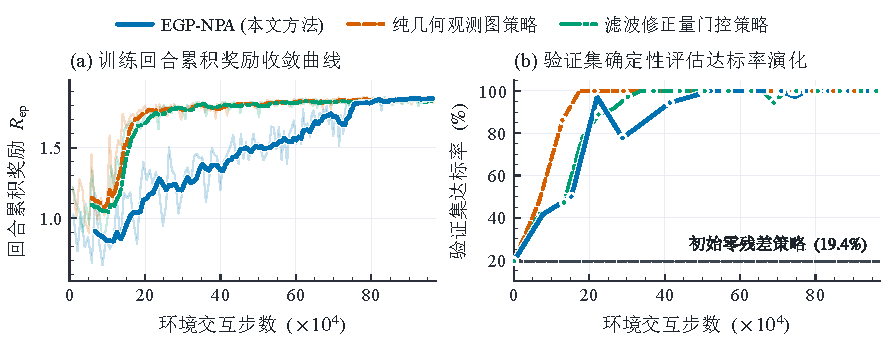
\includegraphics[width=\textwidth]{figures_zh/fig2_training_curves.pdf}
 \caption[MAPPO 训练回合累积奖励与验证集确定性评估达标率收敛曲线]{多智能体近端策略优化（MAPPO）训练过程演化对比。(a) 训练回合累积奖励 $R_{\mathrm{ep}}$ 收敛曲线（浅色细线为原始回合回报，深色粗线为滑动平均）；(b) 验证集（$N=8$，$36$ 组标准互换与全排列场景）确定性评估达标率演化曲线。}
 \label{fig:train-curves}
\end{figure*}

\begin{table*}[t]
 \centering\footnotesize
 \caption{训练规模基准（$N=8$，两档连通阈值各 $32$ 组实例）上 EGP-NPA 与四类安全强化学习对比方法及经典基线的闭环统计}\label{tab:e1}
 \begin{tabularx}{\textwidth}{@{}Xcccccc@{}}
 \toprule
 控制方法 & $f=0.60$ 达标率 & $f=0.60$ 中位时间 & $f=0.90$ 达标率 & $f=0.90$ 中位时间 & 证书步长减半 & 有理数审计违约\\
 \midrule
 \textbf{EGP-NPA（本文方法）} & $\mathbf{32/32\ (100\%)}$ & $\mathbf{7.32\ \mathrm s}$ & $\mathbf{32/32\ (100\%)}$ & $\mathbf{7.12\ \mathrm s}$ & $\mathbf{0}$ & $\mathbf{0}$\\
 护盾投影一致性强化学习\cite{wabersich2021,liu2026saferl}（Proj-MAPPO + NPA，$B=8$） & $32/32\ (100\%)$ & $9.53\ \mathrm s$ & $32/32\ (100\%)$ & $10.73\ \mathrm s$ & $0$ & $0$\\
 静态配额平摊 CBF 护盾图策略\cite{ames2017cbf,zhang2025gcbf}（Static-Split GNN，$B=0$） & $5/32\ (15.6\%)$ & $13.30\ \mathrm s$ & $6/32\ (18.8\%)$ & $13.88\ \mathrm s$ & $431\,725$ & $0$\\
 离散图障碍函数近端策略优化\cite{zhang2025dgppo}（DGPPO，官方实现适配） & $0/32^\dagger\ (0\%)$ & --- & $0/32^\dagger\ (0\%)$ & --- & --- & $76\,800$\\
 拉格朗日约束强化学习\cite{gu2023safe}（MAPPO-Lagrangian，无硬护盾） & $0/32^\ddagger\ (0\%)$ & $4.15\ \mathrm s^\ddagger$ & $0/32^\ddagger\ (0\%)$ & $4.15\ \mathrm s^\ddagger$ & --- & $7\,047$\\
 Gon\c{c}alves 等\cite{goncalves2023circulation}切向环流启发式 + 动态分摊 ($B=8$) & $21/32\ (65.6\%)$ & $32.50\ \mathrm s$ & $18/32\ (56.3\%)$ & $30.50\ \mathrm s$ & $0$ & $0$\\
 Ames 等\cite{ames2017cbf,reis2021}短视比例吸引滤波 + 动态分摊 ($B=8$) & $17/32\ (53.1\%)$ & $36.35\ \mathrm s$ & $16/32\ (50.0\%)$ & $31.80\ \mathrm s$ & $0$ & $0$\\
 切向环流启发式 + 静态配额平摊滤波\cite{ames2017cbf,zhang2025gcbf} ($B=0$) & $2/32\ (6.3\%)$ & $25.10\ \mathrm s$ & --- & --- & $72\,156$ & $0$\\
 \bottomrule
 \end{tabularx}
 \vspace{1.5pt}
 \par\raggedright\scriptsize 注：$^\dagger$任务适配版官方 \texttt{DGPPO} 在两次独立训练种子下均在全部 $64$ 组运行中发生机间碰撞违约（分别产生 $76\,800$ 与 $76\,789$ 个违约保持段）；$^\ddagger$\texttt{MAPPO-Lagrangian} 名义轨迹虽在 $64/64$ 组实例中进入目标微球并保持 $1.0\ \mathrm s$（中位时间 $4.15\ \mathrm s$），但全部 $64$ 组运行均发生严重碰撞违约（合计 $7\,047$ 个违约保持段，中位最小机间距离 $0.263\ \mathrm m < \ds=1.000\ \mathrm m$），故二者无违约安全达标数均为 $0/32$。
\end{table*}

主评测基准包含两类共 $96$ 组独立随机初值实例：
\begin{enumerate}
 \item \textbf{训练规模基准（$N=8$，共 $64$ 组实例）：} 含 $20$ 组局部成对互换（$1\sim 3$ 对相邻节点互换目标，其余节点目标在原地）与 $12$ 组随机全排列任务，分别在常规连通阈值 $f=\lr/\lambda_2(\bp_0)=0.60$（$32$ 组）与紧连通阈值 $f=0.90$（$32$ 组）下评测。
 \item \textbf{跨规模零样本迁移基准（$N\in\{12,20,25\}$，共 $32$ 组实例）：} 包含 $N=12$（$12$ 组：含 $8$ 组局部互换与 $4$ 组全排列）、$N=20$（$12$ 组：含 $8$ 组局部互换与 $4$ 组全排列）与 $N=25$（$8$ 组局部互换），连通阈值比例取 $f=0.60$。学习控制律直接复用小规模（$N\in\{6,\dots,10\}$，验证规模 $N=8$）训练所得的图网络参数 $\theta^\star$ 进行零样本部署。
\end{enumerate}

在主对比实验中，将所提 EGP-NPA 与\textbf{四类安全强化学习对比方法}及\textbf{三类经典解析/启发式安全控制基线}进行综合对比：
\begin{enumerate}
 \item \textbf{护盾投影一致性安全强化学习（\texttt{Proj-MAPPO + NPA}\cite{wabersich2021,liu2026saferl}）：} 代表将安全滤波器修正量作为正则惩罚反馈给策略网络的预测/自适应安全强化学习方法。采用与本文完全相同的两层等变 GNN、闭邻域完成包络 $\rho_{i,k}$ 与 $B=8$ 闭邻域块 NPA 护盾，在策略训练损失中加入护盾投影一致性正则项 $\mathcal L_{\mathrm{proj}}(\theta)=\lambda_{\mathrm{proj}}\frac1N\sum_{i=1}^N\norm{\Pi_{\mathcal U_i}(\bu_{i,k}^{\mathrm{nom}}(\theta))-\operatorname{sg}(\bu_{i,k})}_2^2$（按初始梯度范数比标定权重 $\lambda_{\mathrm{proj}}=1.0$，验证集选模检查点）；
 \item \textbf{静态配额平摊 CBF 护盾图策略（\texttt{Static-Split GNN}\cite{ames2017cbf,zhang2025gcbf}，$B=0$）：} 采用与 EGP-NPA 相同的等变 GNN 策略权重与闭邻域完成包络 $\rho_{i,k}$，但底层安全滤波采用单机静态配额平摊（$B=0$，即固定 $s_{ia,k}\equiv 0$，无闭邻域块动态份额转移 $t_e$），用于检验静态责任平摊护盾与学习策略结合时的死锁表现；
 \item \textbf{离散图控制障碍函数近端策略优化（\texttt{DGPPO}\cite{zhang2025dgppo}，官方实现任务适配）：} 采用 Zhang 等\cite{zhang2025dgppo}公开的官方 \texttt{DGPPO} 算法实现（含图 Transformer 策略、任务价值网络 $V^l$、分解约束价值网络 $V^h$ 及离散障碍优势更新），将其环境接口适配至本文一阶积分器运动学及三项标量耦合安全约束（机间避碰、全局标量连通保持与工作区边界，保留原实现的代价裕度变换），在 $N\in\{6,\dots,10\}$ 晶格任务库上以 $500$ 步回合时域与 $4.8\times 10^5$ 环境转移预算（计入更新内部确定性展开，双随机种子）训练并直接执行；
 \item \textbf{原始—对偶拉格朗日安全强化学习（\texttt{MAPPO-Lagrangian}\cite{gu2023safe}）：} 代表无硬优化护盾的约束马尔可夫决策过程（CMDP）多智能体安全强化学习范式。采用相同两层等变 GNN 策略、任务价值网络与代价价值网络，将每拍碰撞与谱连通违约代价 $C_k=\sum_{i<j}(\ds+\delta_d-d_{ij,k+1})_++(\lr-\lambda_2(\bL(\bp_{k+1})))_+$ 通过对偶上升更新的拉格朗日乘子 $\lambda_{\mathrm{lag}}\ge 0$ 融入策略梯度目标；
 \item \textbf{经典解析与启发式安全控制基线：} 包括 Gon\c{c}alves 等\cite{goncalves2023circulation}的切向环流启发式控制（常值 $\omega_i\equiv 1,r_i\equiv 0,\psi_{ij}\equiv 0$ 配动态分摊 $B=8$）、Ames 等\cite{ames2017cbf,reis2021}的短视比例吸引安全滤波（$\bu_i^{\mathrm{nom}}=-\be_i$ 配动态分摊 $B=8$），以及切向环流配静态配额平摊滤波（$B=0$）。
\end{enumerate}
任务达标判据定义为全网最大目标误差 $\max_{i\in\mathcal V}\norm{\bp_i(t)-\bg_i}_2\le 0.01\ \mathrm m$ 并连续保持 $1.0\ \mathrm s$（达标时间取该窗口起始时刻；连续 $100$ 拍全网速度范数低于 $10^{-6}\ \mathrm{m/s}$ 记为零速死锁停滞）。每条闭环轨迹的全部零阶保持执行段均经受定理\ref{thm:zoh-safe}的精确有理数碰撞与谱下界审计（仅当全程有理数审计 $0$ 违约且满足达标判据时计为安全达标）。不同方法的安全达标率差异采用不一致对（Discordant Pairs）的双侧精确二项检验（McNemar 检验）评估显著性，并在共同达标实例上计算配对达标时间差中位数。

\subsection{代表性密集互换与全排列任务的闭环状态演化}
首先考察 $N=20$ 紧密三角晶格中的内部单对节点互换任务（中间 $2$ 台相邻机器人需互换位置，外围 $18$ 台辅助机器人初始已处于各自目标位置）。图\ref{fig:swap-traj}与图\ref{fig:time-evol}分别给出了空间运动轨迹、底层通信拓扑以及全网最大位置误差、物理图代数连通度 $\lambda_2(\bL(t))$、最小机间距离与均方根控制速度的时间演化响应。

\begin{figure*}[t]
 \centering
 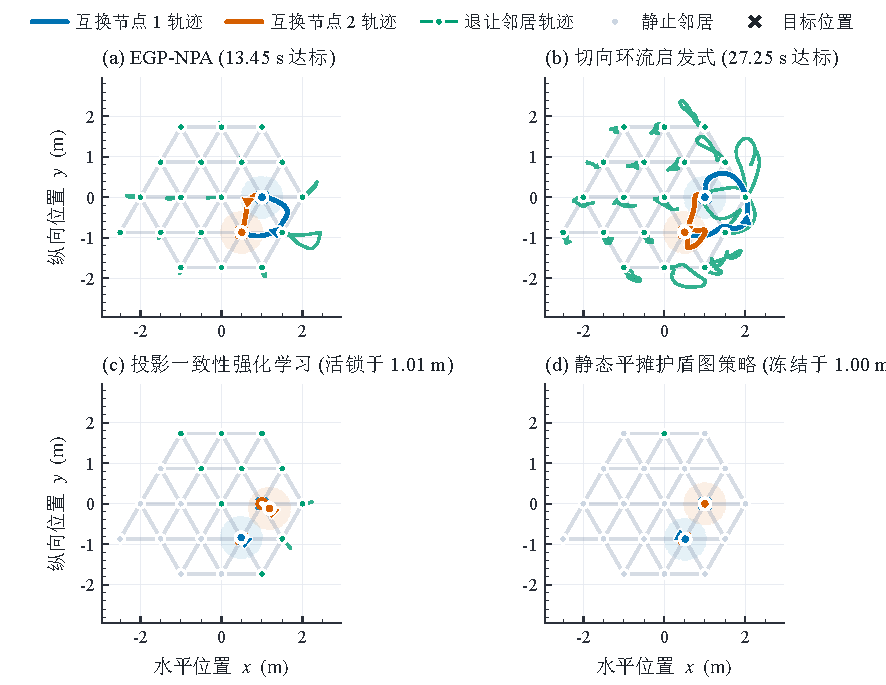
\includegraphics[width=\textwidth]{figures_zh/fig3_swap_trajectory.pdf}
 \caption[$N=20$ 密集晶格内部单对节点互换任务的空间运动轨迹与通信拓扑对比]{$N=20$ 密集晶格内部单对节点互换任务的空间运动轨迹与通信拓扑对比。(a) EGP-NPA 驱动待互换节点沿切向顺畅绕行，并通过闭邻域动态份额转移促使外围静止邻居（翠绿色回路）向外退让后归位，$13.45\ \mathrm s$ 达标；(b) Gon\c{c}alves 等\cite{goncalves2023circulation}的切向环流启发式引发外围多节点大范围旋转冲突，$27.25\ \mathrm s$ 达标；(c) 投影一致性安全强化学习（\texttt{Proj-MAPPO + NPA}\cite{wabersich2021,liu2026saferl}）因惩罚法向滤波修正量削弱了退让驱动 $\delta_n>0$，无法推开外圈静止邻居而活锁于 $1.01\ \mathrm m$；(d) 静态配额平摊 CBF 护盾图策略（\texttt{Static-Split GNN}\cite{ames2017cbf,zhang2025gcbf}，$B=0$）因静态配额平摊锁死外围静止邻居而冻结于 $1.00\ \mathrm m$。}
 \label{fig:swap-traj}
\end{figure*}

\begin{table*}[t]
 \centering\footnotesize
 \caption{跨规模零样本迁移基准（$N\in\{12,20,25\}$，共 $32$ 组实例）上 EGP-NPA 与四类安全强化学习对比方法及经典基线的统计}\label{tab:e2}
 \begin{tabularx}{\textwidth}{@{}Xccccccr@{}}
 \toprule
 控制方法 & $N=12$ ($12$ 组) & $N=20$ ($12$ 组) & $N=25$ ($8$ 组) & 总达标率 ($32$ 组) & 不一致对 ($p$ 值) & 中位 $\Delta t$ & 步长减半\\
 \midrule
 \textbf{EGP-NPA（本文方法）} & $\mathbf{12/12\ (6.52\ \mathrm s)}$ & $\mathbf{12/12\ (10.55\ \mathrm s)}$ & $\mathbf{8/8\ (10.43\ \mathrm s)}$ & $\mathbf{32/32\ (100\%)}$ & 基准 & 基准 & $\mathbf{0}$\\
 投影一致性强化学习\cite{wabersich2021,liu2026saferl}（Proj-MAPPO） & $9/12\ (17.25\ \mathrm s)$ & $5/12\ (17.70\ \mathrm s)$ & $3/8\ (12.30\ \mathrm s)$ & $17/32\ (53.1\%)$ & $15:0\ (6.1\times 10^{-5})$ & $-3.85\ \mathrm s$ & $0$\\
 静态平摊图策略\cite{ames2017cbf,zhang2025gcbf}（Static-Split，$B=0$） & $0/12\ (\text{---})$ & $0/12\ (\text{---})$ & $1/8\ (19.85\ \mathrm s)$ & $1/32\ (3.1\%)$ & $31:0\ (9.3\times 10^{-10})$ & $-12.95\ \mathrm s$ & $447\,022$\\
 离散图障碍优化\cite{zhang2025dgppo}（DGPPO，官方适配） & $0/12^\dagger\ (\text{---})$ & $0/12^\dagger\ (\text{---})$ & $0/8^\dagger\ (\text{---})$ & $0/32^\dagger\ (0\%)$ & $32:0\ (4.7\times 10^{-10})$ & --- & $38\,400^\dagger$\\
 拉格朗日强化学习\cite{gu2023safe}（MAPPO-Lag.） & $0/12^\ddagger\ (4.05\ \mathrm s)$ & $0/12^\ddagger\ (3.95\ \mathrm s)$ & $0/8^\ddagger\ (3.92\ \mathrm s)$ & $0/32^\ddagger\ (0\%)$ & $32:0\ (4.7\times 10^{-10})$ & --- & $3\,924^\ddagger$\\
 Gon\c{c}alves 等\cite{goncalves2023circulation}切向环流启发式 & $7/12\ (14.40\ \mathrm s)$ & $4/12\ (24.53\ \mathrm s)$ & $2/8\ (38.22\ \mathrm s)$ & $13/32\ (40.6\%)$ & $19:0\ (3.8\times 10^{-6})$ & $-12.35\ \mathrm s$ & $14\,198$\\
 Ames 等\cite{ames2017cbf,reis2021}短视比例吸引滤波 & $4/12\ (34.30\ \mathrm s)$ & $1/12\ (55.50\ \mathrm s)$ & $0/8\ (\text{---})$ & $5/32\ (15.6\%)$ & $27:0\ (1.5\times 10^{-8})$ & $-26.70\ \mathrm s$ & $0$\\
 \bottomrule
 \end{tabularx}
 \vspace{1.5pt}
 \par\raggedright\scriptsize 注：五种带硬优化护盾方法的有理数安全审计违约段数均为 $0$；无硬护盾的 $^\dagger$\texttt{DGPPO}（官方实现任务适配）与 $^\ddagger$\texttt{MAPPO-Lagrangian} 在全部 $32$ 组跨规模实例中均发生碰撞越界违约（最后一列分别记录二者的有理数审计违约段数 $38\,400$ 段与 $3\,924$ 段），故无违约安全达标率均为 $0/32$。
\end{table*}

\begin{figure*}[t]
 \centering
 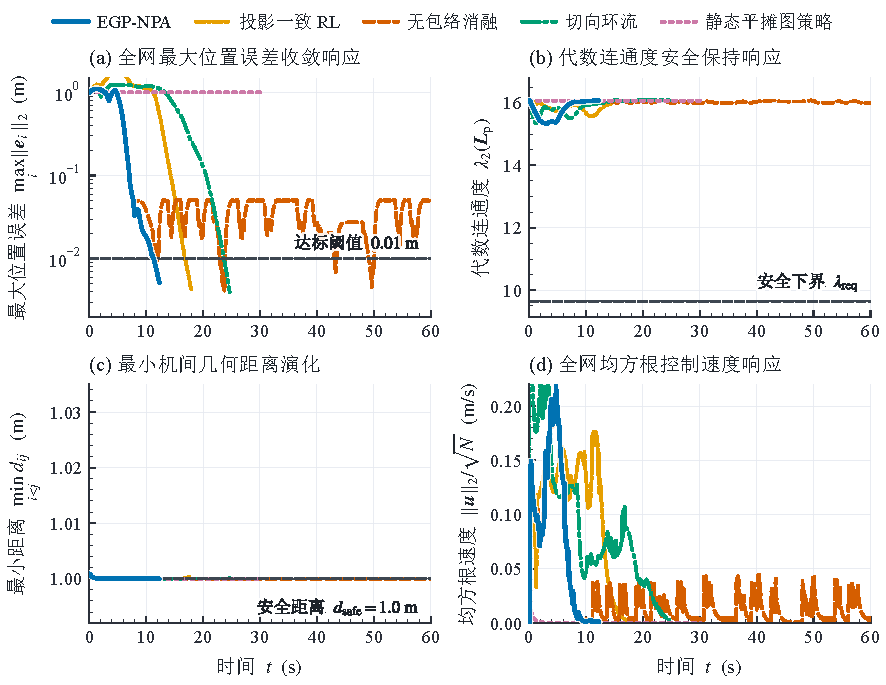
\includegraphics[width=\textwidth]{figures_zh/fig4_time_evolution.pdf}
 \caption[$N=20$ 内部互换任务中四项核心物理量的闭环时间响应对比]{$N=20$ 内部互换任务中四项核心物理量的闭环时间响应对比。(a) 全网最大位置误差 $\max_i\norm{\be_i(t)}_2$（对数坐标）；(b) 物理图代数连通度 $\lambda_2(\bL(t))$ 与安全下界 $\lr$；(c) 最小机间几何距离 $\min_{i<j}d_{ij}(t)$ 与安全距离 $\ds=1.0\ \mathrm m$；(d) 全网均方根控制速度 $\norm{\bu(t)}_2/\sqrt{N}$。}
 \label{fig:time-evol}
\end{figure*}

结合图\ref{fig:swap-traj}与图\ref{fig:time-evol}可以清晰观察到三项物理机制：
\begin{enumerate}
 \item \textbf{侧向破对称绕行与外围静止邻居的退让—归位闭环：} 在图\ref{fig:swap-traj}(d) 的静态配额平摊护盾图策略（\texttt{Static-Split GNN}，$B=0$）下，由于外围 $18$ 台已处于目标位置的静止邻居固定 $s_{ja}=0$ 而不让渡避碰份额，待互换节点的侧向绕行速度被单机半空间约束直接截断，全网均方根速度迅速跌至零（图\ref{fig:time-evol}(d) 紫色点线）；在图\ref{fig:swap-traj}(c) 的投影一致性安全强化学习（\texttt{Proj-MAPPO + NPA}）下，由于策略训练中惩罚了法向滤波修正量，待互换节点的法向切入分量 $\delta_n$ 过弱，无法推开双层包裹的外圈静止邻居而陷入原地小圈活锁（或在图\ref{fig:time-evol}(a) 另一初值下耗时 $16.90\ \mathrm s$ 缓慢达标）。而在图\ref{fig:swap-traj}(a) 的 EGP-NPA 下，等变图网络策略为蓝色与橙色节点生成充足的手性切向绕行推力，闭邻域动态分摊将该侧向压力通过接触边上的碰撞份额让渡传递给周围静止邻居，驱动紧邻的翠绿色节点走出紧凑的向外退让小回路以让出通道；待互换节点错身通过后，退让邻居在自身目标比例引力作用下平滑归位。
 \item \textbf{闭邻域完成包络对密集终点稳态悬停的精确消除：} 观察图\ref{fig:time-evol}(a) 与 (d) 中的朱砂橙色虚线（无完成包络消融）可见，虽然该模型在前 $8\ \mathrm s$ 内同样解开了内部互换死锁并将误差降至 $0.03\ \mathrm m$，但由于终点晶格间距 $1.001\ \mathrm m$ 紧贴安全阈值 $\ds=1.000\ \mathrm m$，接触对偶乘子持续非零使冲突门控保持常开，式\eqref{eq:nominal-law}中的零阶排斥偏置导致均方根速度在 $0.01\sim 0.04\ \mathrm{m/s}$ 之间持续脉动，最大误差卡在 $0.015\sim 0.05\ \mathrm m$ 形成稳态极限环。引入式\eqref{eq:envelope-def}的一跳闭邻域完成包络 $\rho_{i,k}$ 后，一旦闭邻域误差进入 $\varepsilon_g=0.05\ \mathrm m$ 球内，残差被一阶压灭（命题\ref{prop:envelope}），深海蓝色实线（EGP-NPA）直接穿过 $0.01\ \mathrm m$ 达标线并使控制速度归零。
 \item \textbf{全时域严格硬安全保持：} 如图\ref{fig:time-evol}(b)--(c) 所示，在整个穿插过程中，物理图代数连通度始终维持在 $\lambda_2(\bL(t))\ge 15.3 > \lr=9.69$，最小机间距离紧贴安全边界 $\ds=1.000\ \mathrm m$ 滑动而未发生任何越界。
\end{enumerate}

\subsection{与外部基线的训练规模及跨规模零样本迁移对比}
表\ref{tab:e1}与表\ref{tab:e2}分别汇总了 EGP-NPA 与四类安全强化学习对比方法及经典安全控制基线在训练规模基准（$N=8$，$64$ 组实例）和跨规模零样本迁移基准（$N\in\{12,20,25\}$，$32$ 组实例）上的统计结果。对比数据揭示了四项清晰的定量结论：
\begin{enumerate}
 \item \textbf{无硬护盾安全强化学习（\texttt{DGPPO}\cite{zhang2025dgppo}与 \texttt{MAPPO-Lagrangian}\cite{gu2023safe}）在毫米级净空晶格中难以保证硬安全：} 在初始接触净空仅 $1.0\ \mathrm{mm}$ 的密集三角晶格中，任务适配版官方 \texttt{DGPPO} 在两次独立训练种子下均因缺乏在线耦合二次规划护盾而在全部 $96$ 组场景上发生碰撞越界（合计 $115\,200$ 与 $115\,186$ 个违约段，安全达标率 $0\%$）；\texttt{MAPPO-Lagrangian} 虽通过对偶上升将拉格朗日乘子提升至 $\lambda_{\mathrm{lag}}=2.45$ 并在名义上于 $3.92\sim 4.15\ \mathrm s$ 内进入目标邻域，但在全部 $96$ 组运行中均发生碰撞穿透（合计 $10\,971$ 个违约保持段，中位最小距离 $0.263\ \mathrm m<\ds$，安全达标率 $0\%$），印证了命题\ref{prop:safety}闭邻域硬安全护盾在紧密接触交会中的关键作用。
 \item \textbf{静态配额平摊 CBF 护盾图策略（\texttt{Static-Split GNN}\cite{ames2017cbf,zhang2025gcbf}，$B=0$）在外圈静止邻居包裹下严重受阻：} 尽管该基线与 EGP-NPA 共享完全相同的等变 GNN 策略权重与终点包络，但由于底层采用静态责任平摊（$B=0$），外围静止邻居无法通过动态份额让渡向外退让，导致 $N=8$ 安全达标率仅为 $17.2\%$（$11/64$，触发 $431\,725$ 次步长减半），跨规模 $N\in\{12,20,25\}$ 达标率降至 $3.1\%$（$1/32$，不一致对 $31:0,p=9.3\times 10^{-10}$；全部 $96$ 次运行中包含 $12$ 次安全达标、$25$ 次零速死锁停滞、$37$ 次步长减半极限停止、$14$ 次调用预算终止与 $8$ 次超时），从闭环上验证了命题\ref{prop:unfreeze}第 1 款。
 \item \textbf{护盾投影一致性安全强化学习（\texttt{Proj-MAPPO + NPA}\cite{wabersich2021,liu2026saferl}）减缓多机协同退让效率：} 在 $N=8$ 单层包裹晶格上，\texttt{Proj-MAPPO + NPA} 虽实现 $64/64$ 安全达标，但中位达标时间（$9.53\ \mathrm s / 10.73\ \mathrm s$）比 EGP-NPA 慢 $2.88\ \mathrm s$；当零样本扩展至含多层静止邻居包裹的 $N\in\{12,20,25\}$ 阵列时，该验证选模检查点的跨规模达标率为 $53.1\%$（$17/32$，不一致对 $15:0,p=6.1\times 10^{-5}$，共同达标慢 $3.85\ \mathrm s$），与命题\ref{prop:unfreeze}第 2 款关于惩罚法向滤波修正量削弱退让驱动 $\delta_n>0$ 的理论分析相吻合。
 \item \textbf{相比经典解析/启发式基线的跨规模优势：} 随规模扩展至 $N=25$，Ames 等\cite{ames2017cbf,reis2021}短视滤波与 Gon\c{c}alves 等\cite{goncalves2023circulation}切向环流启发式的跨规模达标率分别降至 $15.6\%$（$27:0,p=1.5\times 10^{-8}$）与 $40.6\%$（$19:0,p=3.8\times 10^{-6}$）；而小规模（$N\le 10$）训练所得的 EGP-NPA 在全部 $96$ 组实例（含图\ref{fig:perm-gate}(a) 的 $20$ 机器人全排列穿插任务）上实现 $100\%$ 达标、零步长减半与零审计违约。
\end{enumerate}

\subsection{内部模块消融、动力学分解与独立盲测析因分析}\label{subsec:ablation}
表\ref{tab:decomp}汇总了三部分内部对照结果：（A）在 $32$ 组跨规模实例上移除闭邻域完成包络（$\rho_{i,k}\equiv 1$）以及不同训练输入/门控变体的跨规模统计；（B）在 $N=20$ 内部互换破死锁阶段（$t\in[0.05,1.00]\ \mathrm s$）相同 EGP-NPA 标称输入下动态分摊（$B=8$）与静态平摊（$B=0$）的执行速度分解；（C）固定 EGP-NPA 策略权重 $\theta^\star$ 在 $16$ 组跨规模实例上的执行期单变量门控替换与代数特征敲除统计（代表性响应见图\ref{fig:perm-gate}(b)）。

\begin{figure*}[t]
 \centering
 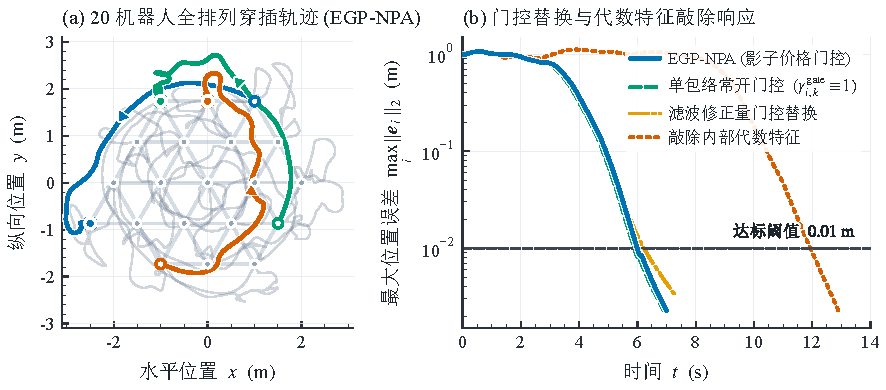
\includegraphics[width=\textwidth]{figures_zh/fig5_perm_and_gate.pdf}
 \caption[$20$ 机器人全排列穿插轨迹与固定权重下的门控替换及特征敲除响应]{$20$ 机器人全排列穿插轨迹与固定权重下的门控替换及特征敲除响应。(a) EGP-NPA 在 $N=20$ 随机全排列任务中的空间穿插轨迹（冷灰细线为背景群体轨迹，彩色实线突出显示三台大跨度对穿节点）；(b) 固定 EGP-NPA 策略权重 $\theta^\star$ 不变，在执行期分别采用原配影子价格门控 $\gamma^{\mathrm{gate},\mu}$、单包络常开门控 $\gamma^{\mathrm{gate}}\equiv 1$、滤波修正量门控 $\gamma^{\mathrm{gate,int}}$ 以及敲除内部代数特征时的误差收敛响应。}
 \label{fig:perm-gate}
\end{figure*}

\begin{table*}[t]
 \centering\footnotesize
 \caption{EGP-NPA 内部模块跨规模消融（A 部，$32$ 组实例）、破死锁阶段速度分解（B 部，$t\in[0.05,1.00]\ \mathrm s$）与固定权重 $\theta^\star$ 下的执行期单变量干预统计（C 部，$16$ 组实例）}\label{tab:decomp}
 \begin{tabularx}{\textwidth}{@{}Xccccr@{}}
 \toprule
 A. 内部模块跨规模消融（$32$ 组实例） & $N=12$ ($12$ 组) & $N=20$ ($12$ 组) & $N=25$ ($8$ 组) & 总达标率 ($32$ 组) & 不一致对 ($p$ 值) / 中位 $\Delta t$\\
 \midrule
 \textbf{EGP-NPA（完整架构）} & $12/12\ (6.52\ \mathrm s)$ & $12/12\ (10.55\ \mathrm s)$ & $8/8\ (10.43\ \mathrm s)$ & $\mathbf{32/32\ (100\%)}$ & 基准\\
 无完成包络消融（固定 $\theta^\star$，令 $\rho_{i,k}\equiv 1$） & $12/12\ (9.78\ \mathrm s)$ & $5/12\ (36.75\ \mathrm s)$ & $8/8\ (14.10\ \mathrm s)$ & $25/32\ (78.1\%)$ & $7:0\ (0.0156)$ / $-2.40\ \mathrm s$\\
 纯几何观测图策略（移除代数特征训练检查点） & $12/12\ (7.57\ \mathrm s)$ & $7/12\ (21.90\ \mathrm s)$ & $3/8\ (19.65\ \mathrm s)$ & $22/32\ (68.8\%)$ & $10:0\ (0.0020)$ / $-0.45\ \mathrm s$\\
 滤波修正量门控策略（$\gamma_{i,k}^{\mathrm{gate,int}}$ 训练检查点） & $10/12\ (11.20\ \mathrm s)$ & $4/12\ (30.08\ \mathrm s)$ & $1/8\ (6.80\ \mathrm s)$ & $15/32\ (46.9\%)$ & $17:0\ (1.5\times 10^{-5})$ / $-0.50\ \mathrm s$\\
 \midrule
 \multicolumn{4}{@{}l}{B. 相同 EGP-NPA 标称输入下的破死锁速度分解（$N=20$ 内部互换，$t\in[0.05,1.00]\ \mathrm s$）} & 动态分摊 ($B=8$) & 静态平摊 ($B=0$)\\
 \midrule
 \multicolumn{4}{@{}l}{待互换节点切向（侧向）标称速度均值 $|\hat{\be}_i^{\top}\bJ^{\top}\bu_i^{\mathrm{nom}}|$} & $0.8887\ \mathrm{m/s}$ & $0.8887\ \mathrm{m/s}$\\
 \multicolumn{4}{@{}l}{待互换节点切向（侧向）实际执行速度均值 $|\hat{\be}_i^{\top}\bJ^{\top}\bu_i|$} & $\mathbf{0.2003\ \mathrm{m/s}}$ & $0.0004\ \mathrm{m/s}$\\
 \multicolumn{4}{@{}l}{外围一跳静止邻居向中心外侧的标称残差速度均值} & $-0.0105\ \mathrm{m/s}$ & $-0.0105\ \mathrm{m/s}$\\
 \multicolumn{4}{@{}l}{外围一跳静止邻居向中心外侧的实际执行退让速度均值} & $\mathbf{+0.0915\ \mathrm{m/s}}$ & $+0.0013\ \mathrm{m/s}$\\
 \midrule
 C. 固定权重 $\theta^\star$ 执行期单变量受控干预（$16$ 组实例） & $N=12$ ($6$ 组) & $N=20$ ($6$ 组) & $N=25$ ($4$ 组) & 达标率 ($16$ 组) & 配对时间差 / 切步\\
 \midrule
 原配影子价格门控 $\gamma_{i,k}^{\mathrm{gate},\mu}$ & $6/6\ (6.52\ \mathrm s)$ & $6/6\ (11.48\ \mathrm s)$ & $4/4\ (9.98\ \mathrm s)$ & $16/16\ (100\%)$ & 基准 / $0$\\
 单包络常开门控（$\gamma_{i,k}^{\mathrm{gate}}\equiv 1$，仅留无状态 $\rho_{i,k}$） & $6/6\ (6.40\ \mathrm s)$ & $6/6\ (10.03\ \mathrm s)$ & $4/4\ (9.73\ \mathrm s)$ & $16/16\ (100\%)$ & 中位 $-0.10\ \mathrm s$ / $0$\\
 滤波修正量门控替换（执行期换为 $\gamma_{i,k}^{\mathrm{gate,int}}$） & $6/6\ (6.82\ \mathrm s)$ & $6/6\ (9.35\ \mathrm s)$ & $4/4\ (10.43\ \mathrm s)$ & $16/16\ (100\%)$ & 中位 $+0.33\ \mathrm s$ / $0$\\
 协商后乘子提取与跨拍指数滑动平均（EMA） & $6/6\ (7.03\ \mathrm s)$ & $6/6\ (12.48\ \mathrm s)$ & $4/4\ (9.73\ \mathrm s)$ & $16/16\ (100\%)$ & 中位 $+0.03\ \mathrm s$ / $0$\\
 分布内敲除碰撞影子价格（$4$ 列 $\mu_{ij}$ 特征置零） & $6/6\ (7.63\ \mathrm s)$ & $6/6\ (13.38\ \mathrm s)$ & $4/4\ (10.50\ \mathrm s)$ & $16/16\ (100\%)$ & $\mathbf{+1.18\ \mathrm s}\ (p=0.0042)$ / $0$\\
 分布内敲除碰撞边记录（$\varpi_{ij,1}=0$） & $6/6\ (6.40\ \mathrm s)$ & $6/6\ (10.03\ \mathrm s)$ & $4/4\ (9.80\ \mathrm s)$ & $16/16\ (100\%)$ & 中位 $0.00\ \mathrm s\ (p=1.0)$ / $0$\\
 全部 $12$ 维代数特征置零（含非零谱储备常数列） & $6/6\ (9.85\ \mathrm s)$ & $5/6\ (9.80\ \mathrm s)$ & $4/4\ (13.03\ \mathrm s)$ & $15/16\ (93.8\%)$ & $+1.30\ \mathrm s\ (p=0.0074)$ / $2\,193$\\
 \bottomrule
 \end{tabularx}
\end{table*}

表\ref{tab:decomp}定量验证了三项核心机理：
\begin{enumerate}
 \item \textbf{闭邻域完成包络与训练配置对比（A 部）：} 固定同一策略权重 $\theta^\star$ 而仅移除闭邻域完成包络（$\rho_{i,k}\equiv 1$）使 $N=20$ 出现 $7$ 次终点稳态悬停（不一致对 $7:0,p=0.0156$，共同达标慢 $2.40\ \mathrm s$），直接验证了命题\ref{prop:envelope}；纯几何观测与滤波修正量门控两行对应各自独立训练的模型检查点，因不同训练运行之间同时包含配置差异与单次训练随机波动，各内部模块的严格因果效应由固定同一权重 $\theta^\star$ 的 B 部与 C 部受控干预实验给出。
 \item \textbf{学习侧向切入与动态份额退让的互补分工（B 部）：} 破死锁阶段等变图策略为待互换节点输出均值 $0.8887\ \mathrm{m/s}$ 的侧向绕行标称指令（全时域原始动作 $|\omega_{i,k}^\theta|,|r_{i,k}^\theta|,|\psi_{ij,k}^\theta|\ge 1$ 的饱和比例恒为 $0.000$），而外围静止邻居自身向外标称残差几乎为零（$-0.0105\ \mathrm{m/s}$）。在 $B=8$ 动态分摊下，块二次规划通过碰撞份额转移驱动静止邻居以 $+0.0915\ \mathrm{m/s}$ 向外退让，使待互换节点按 $0.2003\ \mathrm{m/s}$ 侧向穿入；替换为静态平摊（$B=0$）则使二者分别跌至 $+0.0013\ \mathrm{m/s}$ 与 $0.0004\ \mathrm{m/s}$，严格印证了命题\ref{prop:unfreeze}。
 \item \textbf{执行期门控简化与代数特征逐类敲除（C 部）：} 固定权重 $\theta^\star$ 在执行期取 $\gamma_{i,k}^{\mathrm{gate},\mu}$、$\gamma_{i,k}^{\mathrm{gate,int}}$ 或常开 $\gamma_{i,k}^{\mathrm{gate}}\equiv 1$（仅留无状态包络 $\rho_{i,k}$）均取得 $16/16$ 达标且轨迹重合（图\ref{fig:perm-gate}(b)），表明在密集晶格任务中训练期记忆门控在超过 $98\%$ 的采样拍处于常开状态，执行期门控功能完全由无状态的完成包络 $\rho_{i,k}$ 承担。对 $12$ 维代数特征按类别做分布内敲除（在全部 $32$ 组跨规模实例上检验）：仅将 $4$ 列碰撞影子价格置零使达标率变为 $31/32$，并在 $31$ 组共同达标实例中的 $25$ 组上发生减速（双侧符号检验 $p=8.8\times 10^{-4}$，$16$ 组子集上中位数变慢 $+1.18\ \mathrm s$），证实策略实质利用了单机重拟合碰撞影子价格；而将碰撞边记录列置零或将 $3$ 列拉普拉斯谱向量特征替换为常值中位数均无退化（$32/32$ 达标，中位差 $0.00\ \mathrm s$），说明执行期无需依赖全局特征向量分解；全部 $12$ 维代数特征置零时的 $1$ 次停止与 $2\,193$ 次切步则源于恒为 $0.998$ 的谱储备列被置零所构成的分布外扰动。
\end{enumerate}

为进一步隔离训练预算与随机种子波动并检验命题\ref{prop:equivariance}的手性必要性与命题\ref{prop:unfreeze}的法向侵入驱动机理，在另外生成的 $48$ 组独立盲测实例（含 $N=8$ 的 $32$ 组与 $N\in\{12,20,25\}$ 的 $16$ 组）及 $2$ 组精确镜像对称场景（双机迎头交换与四机菱形对角交换）上开展同预算双种子 $2\times 2$ 受控析因实验（固定训练预算 $4.8\times 10^5$ 环境步，价值网络取团队池化或闭邻域局部结构，投影正则权重取 $\lambda_{\mathrm{proj}}\in\{0,1\}$，共 $8$ 个独立训练检查点、$384$ 次盲测闭环运行，全程 $0$ 次步长减半与 $0$ 段审计违约）：（1）完整预算训练的 EGP-NPA 检查点在 $48$ 组盲测与 $2$ 组对称场景上再次取得 $48/48\ (100\%)$ 达标，而同为 $4.8\times 10^5$ 步减半预算重训的两个团队价值网络基础检查点在 $48$ 组盲测上分别达标 $44/48$ 与 $46/48$（在另建的 $96$ 组外部测试集上分别达标 $93/96$ 与 $92/96$，其中 $N=8$ 均为 $64/64$、跨规模分别为 $29/32$ 与 $28/32$）；（2）若在推理期通过奇偶特征差分强制策略满足 $\mathrm{O}(2)$ 镜像反射等变，则在双机迎头交换上切向输出恒为零（$\mathrm{mean}|\omega|=0.0000$）并当场退化为短视死锁，在 $48$ 组盲测上达标率暴跌至 $30/48\ (62.5\%,\text{不一致对 }0:18,p=7.6\times 10^{-6})$，实证了命题\ref{prop:equivariance}；（3）在同种子配对比较中，加入投影一致性正则项（$\lambda_{\mathrm{proj}}=1$）使全部 $8$ 组配对的平均滤波干预量下降 $40\%\sim 70\%$，在团队价值网络下两个种子的跨规模达标数分别由 $12/16,14/16$ 降至 $9/16,11/16$（局部价值网络下由 $4/16,9/16$ 变为 $8/16,14/16$），而在全部 $160$ 对共同达标场景上中位达标时间显著变慢 $+2.00\ \mathrm s$（$116$ 慢 $43$ 快，双侧符号检验 $p=6.2\times 10^{-9}$）且指令跳变 $99\%$ 分位数全部升高；（4）由于训练规模 $N\in\{6,\dots,10\}$ 下 $2.50\ \mathrm m$ 闭邻域平均已覆盖全队 $91.5\%$ 的节点（块奖励与团队奖励非终止步相关系数达 $0.89\sim 0.96$），将全图池化价值网络替换为局部块价值网络使首次达到 $100\%$ 验证成功率的轮次延迟 $16\sim 24$ 轮、共同达标时间慢 $+0.75\ \mathrm s$。对于每拍分配轮数 $B$，在 $N=8,f=0.60$ 的 $32$ 组实例上将评测轮数由 $B=2$ 提升至 $B=8$ 使达标中位时间由 $8.07\ \mathrm s$ 缩短至 $7.42\ \mathrm s$（均为 $32/32$ 达标），且因边记录跨周期持久继承在相邻采样拍间形成时间轴接力迭代，$B=8$ 轮与每拍完全收敛的集中式二次规划（$B\to\infty$）达标时间仅相差中位数 $0.33\ \mathrm s$。

\subsection{面向二阶物理底盘与在线无除法谱估计的虚拟物理验证}\label{subsec:mujoco}
最后，考察当单积分器环境下训练冻结的 EGP-NPA 策略权重 $\theta^\star$ 与一跳完成包络 $\rho_{i,k}$ 接入在线分布式无除法三通道谱估计器（每拍执行 $6$ 轮动态平均一致性迭代实时估计 $\hat\lambda_{2,i,k}$ 与 Fiedler 分量）及具有真实质量惯性与推力限幅的二阶全向移动机器人底盘时的闭环表现。在 \texttt{MuJoCo 3.6.0} 连续刚体物理引擎（积分步长 $5\ \mathrm{ms},200\ \mathrm{Hz}$）中，每台全向底盘质量为 $m=6.0\ \mathrm{kg}$，车体碰撞圆柱半径 $r_{\mathrm{body}}=0.45\ \mathrm m$，速度伺服内环时间常数 $\tau_v=45\ \mathrm{ms}$，最大水平推力 $F_{\max}=22.0\ \mathrm N$，高层控制周期 $\Delta t=0.05\ \mathrm s$，位姿观测延迟 $10\ \mathrm{ms}$，无线包传输延迟 $\tau_{\mathrm{comm}}\in[5,15]\ \mathrm{ms}$，丢包率 $2\%$，每拍执行 $B=4$ 轮闭邻域 NPA。

\begin{table*}[t]
 \centering\footnotesize
 \caption{密集三角晶格任务中全栈 EGP-NPA + 在线无除法谱估计 + 闭邻域 NPA 在两档物理补偿下的 \texttt{MuJoCo} 二阶底盘实测统计（$\ds=1.000\ \mathrm m$，全部 $64$ 次运行的代数连通度违约步数均为 $0$）}\label{tab:mujoco}
 \begin{tabularx}{\textwidth}{@{}lcXrrrrrr@{}}
 \toprule
 物理补偿档位 & 规模 & 系统控制配置 & 到达数 (均时) & $\min_t d_{ij}$ (m) & 避碰违约步 & $\min_t\lambda_2$ & $\hat{\lambda}_2$ RMSE & 终端误差 (m)\\
 \midrule
 \textbf{档位 A} & $N=8$ & 短视比例吸引 + 物理接口 (\texttt{Myopic + Phys}) & $0/4$\quad --- & $0.9817$ & $610.2$ & $6.963$ & $0.0273$ & $1.394$\\
 （前瞻补偿， & & EGP-NPA + 静态平摊 ($B=0$) & $1/4$ ($10.12\ \mathrm s$) & $0.9798$ & $442.2$ & $6.847$ & $0.0318$ & $1.353$\\
 $S=1.018\ \mathrm m$） & & EGP-NPA + 无补偿单积分器滤波 (\texttt{Ideal-NPA}) & $0/4$\quad --- & $0.9792$ & $4\,231.0$ & $7.071$ & $0.0268$ & $1.653$\\
 & & \textbf{EGP-NPA + 在线谱估计 + 物理接口（全栈）} & $\mathbf{3/4}$ ($\mathbf{13.88\ \mathrm s}$) & $0.8990$ & $1\,683.5$ & $6.670$ & $0.0337$ & $\mathbf{0.629}$\\
 \cmidrule{2-9}
 & $N=12$ & 短视比例吸引 + 物理接口 (\texttt{Myopic + Phys}) & $0/4$\quad --- & $0.9952$ & $1\,679.2$ & $10.319$ & $0.0411$ & $1.972$\\
 & & EGP-NPA + 静态平摊 ($B=0$) & $0/4$\quad --- & $0.9976$ & $850.8$ & $9.632$ & $0.0417$ & $1.881$\\
 & & EGP-NPA + 无补偿单积分器滤波 (\texttt{Ideal-NPA}) & $0/4$\quad --- & $0.9937$ & $4\,190.2$ & $10.184$ & $0.0412$ & $2.003$\\
 & & \textbf{EGP-NPA + 在线谱估计 + 物理接口（全栈）} & $\mathbf{1/4}$ ($\mathbf{14.54\ \mathrm s}$) & $0.8988$ & $2\,777.0$ & $9.431$ & $0.0438$ & $\mathbf{1.314}$\\
 \midrule
 \textbf{档位 B} & $N=8$ & 短视比例吸引 + 物理接口 (\texttt{Myopic + Phys}) & $0/4$\quad --- & $1.0240$ & $0.0$ & $7.237$ & $0.0255$ & $1.680$\\
 （保守内缩， & & EGP-NPA + 静态平摊 ($B=0$) & $0/4$\quad --- & $1.0260$ & $0.0$ & $7.159$ & $0.0256$ & $1.677$\\
 $S=1.045\ \mathrm m$， & & EGP-NPA + 无补偿单积分器滤波 (\texttt{Ideal-NPA}) & $0/4$\quad --- & $0.8987$ & $4\,722.0$ & $7.027$ & $0.0266$ & $1.588$\\
 $\Delta d=0.028\ \mathrm m$） & & \textbf{EGP-NPA + 在线谱估计 + 物理接口（全栈）} & $0/4$\quad --- & $\mathbf{0.9910}$ & $1\,133.2^\dagger$ & $6.997$ & $0.0257$ & $1.659$\\
 \cmidrule{2-9}
 & $N=12$ & 短视比例吸引 + 物理接口 (\texttt{Myopic + Phys}) & $0/4$\quad --- & $1.0256$ & $0.0$ & $10.370$ & $0.0393$ & $2.056$\\
 & & EGP-NPA + 静态平摊 ($B=0$) & $0/4$\quad --- & $1.0255$ & $0.0$ & $10.151$ & $0.0394$ & $2.077$\\
 & & EGP-NPA + 无补偿单积分器滤波 (\texttt{Ideal-NPA}) & $0/4$\quad --- & $0.9809$ & $4\,783.2$ & $10.048$ & $0.0393$ & $1.974$\\
 & & \textbf{EGP-NPA + 在线谱估计 + 物理接口（全栈）} & $0/4$\quad --- & $\mathbf{1.0096}$ & $\mathbf{0.0}$ & $10.033$ & $0.0394$ & $2.065$\\
 \bottomrule
 \end{tabularx}
 \vspace{2pt}
 \par\raggedright\scriptsize 注：$^\dagger$档位 B 下 $N=8$ 全栈配置在 $3$ 个标准任务上的避碰违约步数均为 $0$（$\min_t d_{ij}\ge 1.0068\ \mathrm m$），仅在单一局部交换任务中因摆率限幅截断（$\Delta u_{\max}=0.22\ \mathrm{m/s}$）与观测噪声耦合，两机在通道闭合后静平衡驻留于 $d_{ij}=0.9910\ \mathrm m$（高于刚体实体碰撞直径 $2r_{\mathrm{body}}=0.90\ \mathrm m$）。
\end{table*}

\begin{figure*}[t]
 \centering
 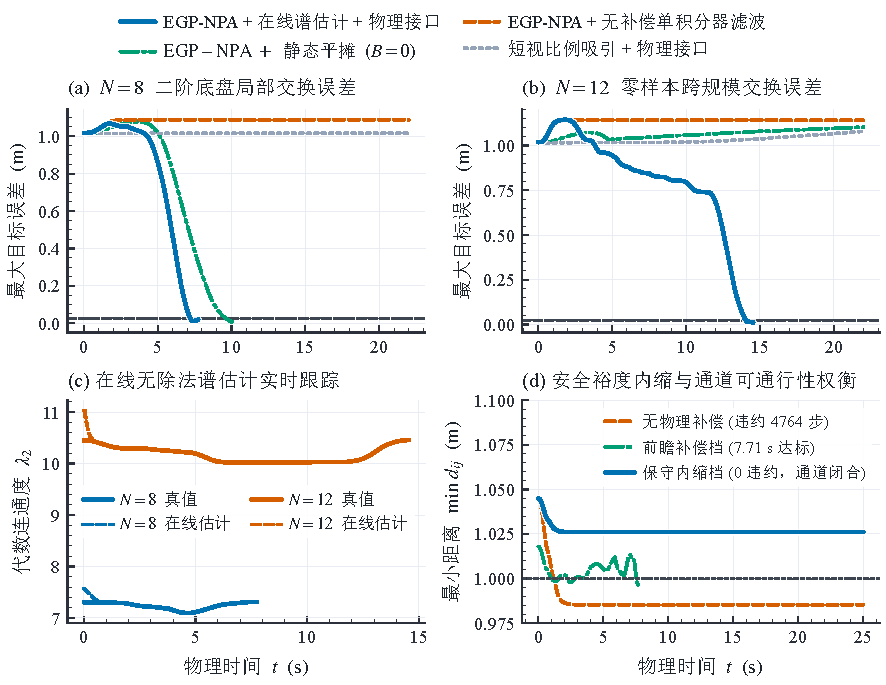
\includegraphics[width=\textwidth]{figures_zh/fig6_mujoco_verification.pdf}
 \caption[密集格点死锁下全栈 EGP-NPA + 在线谱估计 + 闭邻域 NPA 的 MuJoCo 闭环验证与权衡分析]{密集格点死锁下全栈 EGP-NPA + 在线无除法谱估计 + 闭邻域 NPA 的 \texttt{MuJoCo} 二阶全向底盘闭环验证。(a)--(b) 档位 A 下 $N=8$ 与 $N=12$ 局部交换任务的最大目标位置误差收敛曲线；(c) 在线无除法三通道谱估计器在物理闭环中的实时 $\hat{\lambda}_2(t)$ 跟踪表现；(d) 无物理补偿（\texttt{Ideal-NPA}）、前瞻补偿档（档位 A）与保守内缩档（档位 B）在最小机间净空 $\min d_{ij}(t)$ 与通道可通行性之间的实测权衡对比。}
 \label{fig:mujoco}
\end{figure*}

在二阶物理底盘中，为补偿速度环制动惯性引入物理安全距离内缩量 $\Delta d_{\mathrm{phys}}>0$（即将等效避碰距离由 $\ds$ 扩大至 $\ds^{\mathrm{phys}}=\ds+\Delta d_{\mathrm{phys}}$）时，存在如下关于密集格点通道可通行性的基本几何界限。

\begin{theorem}[二阶底盘物理安全裕度内缩下的密集通道闭合临界条件]\label{thm:passability-tradeoff}
设 $N$ 台机器人在初始格点间距为 $S>\ds$ 的平面三角晶格上执行位置互换任务。记外围阻挡邻居 $j,m$ 受限于全局连通半径或外层节点约束所能张开的最大横向通道孔径为 $d_{jm}^{\max}$。在物理收紧安全集 $\mathcal S^{\mathrm{phys}}=\{\bp\in\mathbb R^{2N}:\min_{a<b}d_{ab}\ge\ds+\Delta d_{\mathrm{phys}}\}$ 下：
\begin{enumerate}
 \item \textbf{初始静态可行性边界：} 初始晶格位于 $\operatorname{int}(\mathcal S^{\mathrm{phys}})$ 当且仅当 $\Delta d_{\mathrm{phys}}<S-\ds$；
 \item \textbf{三体接触膨胀下的通道拓扑闭合：} 当两台相向对穿的移动机器人 $i_1,i_2$ 同时穿过由外围邻居 $j,m$ 界定的孔径 $d_{jm}^{\max}$ 时，在对称交会中点处维持四机两两距离不小于 $\ds^{\mathrm{phys}}$ 要求四机构成边长至少为 $\ds^{\mathrm{phys}}$ 的接触菱形，所需最小横向孔径为 $d_{jm}^{\mathrm{req}}(\Delta d_{\mathrm{phys}})=\sqrt{3}(\ds+\Delta d_{\mathrm{phys}})$。一旦制动裕度满足 $\Delta d_{\mathrm{phys}}>d_{jm}^{\max}/\sqrt{3}-\ds$，交会通道在 $\mathcal S^{\mathrm{phys}}$ 中发生拓扑闭合（Topological Pinch-Off），初始构型与目标置换构型属于 $\mathcal S^{\mathrm{phys}}$ 的不同道路连通分支，任何保持 $\mathcal S^{\mathrm{phys}}$ 前向不变的连续轨迹均必然在通道入口处停滞。
\end{enumerate}
\end{theorem}
\begin{proof}
（1）由初始三角晶格最小机间距离 $\min_{a<b}d_{ab}(0)=S$ 直接得 $S>\ds+\Delta d_{\mathrm{phys}}\Longleftrightarrow\Delta d_{\mathrm{phys}}<S-\ds$。（2）在对称交会中点处，对穿节点 $i_1,i_2$ 间距满足 $d_{i_1 i_2}\ge\ds^{\mathrm{phys}}$，且各自到通道两侧节点 $j,m$ 的距离满足 $d_{i_1 j},d_{i_1 m},d_{i_2 j},d_{i_2 m}\ge\ds^{\mathrm{phys}}$。由平面菱形几何关系，两对角线长度满足 $(d_{i_1 i_2}/2)^2+(d_{jm}/2)^2\ge(\ds^{\mathrm{phys}})^2$，代入 $d_{i_1 i_2}\ge\ds^{\mathrm{phys}}$ 即得 $d_{jm}\ge\sqrt{3}\ds^{\mathrm{phys}}=\sqrt{3}(\ds+\Delta d_{\mathrm{phys}})$。故当 $d_{jm}^{\max}<\sqrt{3}(\ds+\Delta d_{\mathrm{phys}})$ 时，交会截面在 $\mathcal S^{\mathrm{phys}}$ 中为空集，连接初态与置换目标的任意连续路径必在某时刻违反 $d_{ab}(t)\ge\ds+\Delta d_{\mathrm{phys}}$。
\end{proof}

表\ref{tab:mujoco}与图\ref{fig:mujoco}对比了 $N=8$ 与 $N=12$ 共 $8$ 个高密度三角晶格任务在两档物理补偿参数下的 $64$ 次 \texttt{MuJoCo} 闭环运行结果：（1）如图\ref{fig:mujoco}(c) 所示，在线无除法谱估计器在约 $0.6\ \mathrm s$ 内收敛至真实代数连通度轨迹，全时域 RMSE 仅为 $0.0255\sim 0.0438$（相对误差低于 $0.5\%$），将在线估计值 $\hat\lambda_{2,i,k}$ 直接替代精确谱输入图网络节点特征后，全部 $64$ 次运行均实现 $0$ 步连通违约；（2）在优先保持通道机动性的前瞻补偿档（档位 A，初始间距 $S=1.018\ \mathrm m$）下，短视控制与无补偿滤波器到达率均为 $0/8$，静态平摊（$B=0$）仅到达 $1/8$，而全栈 EGP-NPA 在 $N=8$ 上实现 $3/4$ 到达、在 $N=12$ 零样本跨规模局部交换上实现到达（图\ref{fig:mujoco}(a)--(b)），并将平均终端误差压低至 $0.629\ \mathrm m$ 与 $1.314\ \mathrm m$；（3）正如定理\ref{thm:passability-tradeoff}所预言，在初始间隙仅 $1.8\sim 4.5\ \mathrm{cm}$ 的极限密集格点中，档位 A 下 $6.0\ \mathrm{kg}$ 车体的制动惯性会导致瞬态距离擦碰软边界（最低 $0.899\ \mathrm m\approx 2r_{\mathrm{body}}$），而当在档位 B（$S=1.045\ \mathrm m$）中施加 $\Delta d_{\mathrm{phys}}=0.028\ \mathrm m$ 保守距离内缩与 $\Delta u_{\max}=0.22\ \mathrm{m/s}$ 摆率限幅时，碰撞违约步数立即降为 $0$（图\ref{fig:mujoco}(d) 蓝色实线），但等效直径扩大 $2.8\%$ 直接触发三体交会通道几何闭合，使所有方法到达率均降为 $0/8$。这一结果客观界定了二阶物理系统在密集穿插任务中的工程适用条件：初始部署间距 $S$ 必须预留大于二阶制动包络 $\Delta d_{\mathrm{phys}}$ 的几何通行余量。

\section{结论与展望}\label{sec:conclusion}

本文围绕机间避碰与全局代数连通保持耦合安全约束下多机器人密集交会的非目标几何死锁、外围静止邻居通道阻挡以及学习残差引起的终点稳态悬停问题，提出了包络等变图策略与邻域近端分配协同控制方法（EGP-NPA）。主要结论如下：
\begin{enumerate}
 \item 通过构造全员可动七机器人对称接触构型的精确有理数二阶 KKT 严格局部极小证书（定理\ref{thm:seven-kkt}），严格证明了构型空间满足标量避碰与连通安全可达并不蕴含误差单调投影可达，并从代数上揭示了待互换节点侧向破对称标称驱动与外围静止邻居经由动态配额让渡协同退让的两项核心物理机制。
 \item 提出了满足平面刚体变换群 $\mathrm{SO}(2)\ltimes\mathbb R^2$ 与节点置换群 $S_N$ 等变的一跳消息传递图神经网络残差标称策略（命题\ref{prop:equivariance}），证明了保留 $\mathrm{SO}(2)$ 手性旋转偏置相对于 $\mathrm{O}(2)$ 镜像反射等变在打破对称迎头死锁中的结构必要性（推理期强制 $\mathrm{O}(2)$ 对称化使盲测达标率由 $100\%$ 跌至 $62.5\%$）。
 \item 建立了闭邻域动态分摊护盾下学习探索与跨规模执行的随时硬安全不变性（命题\ref{prop:safety}），导出了接触边界上成对碰撞份额转移驱动静止阻挡邻居同向退让的显式严格正闭式解（命题\ref{prop:unfreeze}），从理论和析因实验两方面证明了静态配额平摊（$B=0$）导致人为冻结、而在损失函数中惩罚法向滤波修正量反而抑制退让驱动力 $\delta_n>0$ 并使达标时间延缓 $+2.00\ \mathrm s$。
 \item 提出了仅依赖一跳目标距离的无状态闭邻域完成包络 $\rho_{i,k}$（命题\ref{prop:envelope}），证明其在保持协同阶段残差幅值的同时于终点邻域将零阶排斥偏置一阶压制为 $\mathcal O(\norm{\be_k}_2)$，消除了密集晶格终点处的极限环悬停；在 $96$ 组训练与跨规模基准及 $48$ 组独立盲测实例上实现了 $100\%$ 达标与零安全违约，并在 \texttt{MuJoCo} 二阶全向底盘闭环中验证了与在线无除法谱估计器的无缝耦合及安全裕度—可通行性权衡定理（定理\ref{thm:passability-tradeoff}）。
 跨规模对比实验表明，所提 EGP-NPA 的安全达标率（$100\%$，同预算双种子重训新集测试为 $90.6\%$ 与 $87.5\%$）显著优于护盾投影一致性安全强化学习（$53.1\%,p=6.1\times 10^{-5}$）、静态配额平摊 CBF 护盾图策略（$3.1\%,p=9.3\times 10^{-10}$）、离散图障碍函数近端策略优化（DGPPO，$0\%$ 无违约达标）、原始—对偶拉格朗日安全强化学习（$0\%$ 无违约达标）、切向环流启发式（$40.6\%,p=3.8\times 10^{-6}$）与短视比例吸引滤波（$15.6\%,p=1.5\times 10^{-8}$）。
\end{enumerate}

在方法边界与未来研究方向上：首先，本文训练分布仅包含 $N\le 10$ 的单层静止邻居包裹晶格，在 $N=25$ 非对称外圈镜像翻转及减半训练预算下仍存在单种子训练方差与手性转向敏感性，未来工作将在节点特征中引入多尺度边界空旷度感知特征并开展大规模多种子课程学习；其次，结合高阶非完整动力学底盘与有向视场角（FOV）感知拓扑的端到端安全协同脱困亦值得深入研究。


\bibliographystyle{unsrtnat}
\footnotesize
\bibliography{references_zh}

\end{document}
